\documentclass[main.tex]{subfiles}
\begin{document}


\section{Модели в двух пространство-время измерениях без взаимодействий}\label{ch17}
\subsection{Двухмерная модель безмассовых бозонов}\label{ch17.1}

Важной мотивацией для нашего перехода от действительных чисел к целым является то, что мы требуем, чтобы детерминированные теории были бесконечно точными. Любая система, основанная на классическом действии, требует действительных чисел для своих основных переменных, но это также вводит ограниченную точность. Если, как можно предположить, предельные физические степени свободы просто образуют биты и байты, то они могут быть только дискретными, а прототипы дискретных систем являются целыми числами. Возможно, позже можно будет заменить их на целые числа с максимальным размером, такие как целые числа деленные с остатком на простое число $p$, $\in\mathbb{Z} / p\mathbb{Z}$.

Вопрос в том, как сформулировать системный подход. Например, как мы подражаем квантовой теории поля? Если такая теория основана на пертурбативных разложениях, можем ли мы имитировать такие разложения в терминах целых чисел? Нет необходимости замечать, что стандартные разложения возмущений кажутся невозможными для дискретных систем, но все еще можно представить различные специальные виды разложений, такие как разложения $1 / N$, где $N$ может быть некоторой характеристикой базовой алгебры.

Мы не будем это проделывать в данной книге, но мы начнем с формулирования систематических подходов. В этой главе мы рассмотрим квантованное поле, полевые переменные которого, разумеется, являются операторами с континуумами собственных значений в действительных числах. Если мы хотим пробиться к теории возмущенных полей, нам сначала нужно понять свободные частицы. Один пример был рассмотрен в разд. \ref{ch15.2}. Это были фермионы. Теперь мы попробуем ввести свободные бозоны.

Такие теории подчиняются линейным уравнениям поля, таким как

\begin{equation}\label{17.1}
	\partial_{t}^{2} \phi(\vec{x}, t)=\sum_{i=1}^{d} \partial_{i}^{2} \phi(\vec{x}, t)-m^{2} \phi(\vec{x}, t)
\end{equation}

В случае фермионов нам удалось до некоторой степени сформулировать безмассовый случай в трех пространственных измерениях (раздел \ref{ch15.2.3}), но применение теории $PQ$ к бозонным полям в более чем двух измерениях не было успешным. Проблема в том, что уравнения, такие как уравнение (\ref{17.1}) трудно применить к целым числам, даже если мы можем заполнить промежутки между целыми числами генераторами смещений.

В нашем поиске систем, где это можно сделать, мы выбрали в качестве компромисса безмассовые поля только в одном пространственно-подобном измерении. Причина, почему этот частный случай может быть обработан с помощью теории $PQ$, заключается в том, что уравнение поля (\ref{17.1}), можно свести к уравнениям первого порядка, различая левые и правые двигатели. Давайте сначала кратко подведем итоги квантовой теории континуума для этого случая.





\subsubsection{Вторично-квантованные безмассовые бозоны в двух измерениях}\label{ch17.1.1}

Мы рассматриваем одно, скалярное, невзаимодействующее, бесмассовое поле $q(x, t)$. И $x$, и $t$ одномерны. Тогда лагранжиан и гамильтониан:

\begin{equation}\label{17.2}
\mathcal{L}=\frac{1}{2}\left(\partial_{t} q^{2}-\partial_{x} q^{2}\right) ; \quad H_{\mathrm{op}}=\int \mathrm{d} x\left(\frac{1}{2} p^{2}+\frac{1}{2} \partial_{x} q^{2}\right)
\end{equation}

где мы используем символ $p(x)$ для обозначения канонического поля импульса, связанного со скалярным полем $q(x)$, которое при отсутствии взаимодействия подчиняется $p(x)=\partial_{t} q(x)$. Поля $q(x)$ и $p(x)$ являются операторными полями. Правила переключения на равное время, как обычно:

\begin{equation}\label{17.3}
[q(x), q(y)]=[p(x), p(y)]=0 ; \quad[q(x), p(y)]=i \delta(x-y)
\end{equation}

Рассмотрим переменную времени в $q(x, t)$ и $p(x, t)$ нотации Гейзенберга. Тогда у нас есть уравнения поля:

\begin{equation}\label{17.4}
\partial_{t}^{2} q=\partial_{x}^{2} q
\end{equation}

и решение уравнений поля можно записать следующим образом:

\begin{equation}\label{17.5}
a^{L}(x, t)=p(x, t)+\partial_{x} q(x, t)=a^{L}(x+t)
\end{equation}

\begin{equation}\label{17.6}
a^{R}(x, t)=p(x, t)-\partial_{x} q(x, t)=a^{R}(x-t)
\end{equation}

Уравнения заставляют операторы $a^{L}$ двигаться влево и $a^{R}$ вправо. С точки зрения этих переменных, гамильтониан (в данный момент времени $t$ ) - выглядит так

\begin{equation}\label{17.7}
H_{\mathrm{op}}=\int \mathrm{d} x \frac{1}{4}\left(\left(a^{L}(x)\right)^{2}+\left(a^{R}(x)\right)^{2}\right)
\end{equation}

Правила коммутации для $a^{L, R}$ таковы:

$\left[a^{L}, a^{R}\right]=0, \quad\left[a^{L}\left(x_{1}\right), a^{L}\left(x_{2}\right)\right]=2 i \delta^{\prime}\left(x_{1}-x_{2}\right)$
\begin{equation}\label{17.8}
\left[a^{R}\left(x_{1}\right), a^{R}\left(x_{2}\right)\right]=-2 i \delta^{\prime}\left(x_{1}-x_{2}\right)
\end{equation}

где $\delta^{\prime}(z)=\frac{\partial}{\partial z} \delta(z)$
Теперь приступим к преобразованию Фурье по пространственной координате, перейдя к моментальным переменным пространства $k,$ и вычтем энергию вакуума. Мы находимся в импульсном пространстве (обратите внимание, что мы ограничиваемся позитивными значениями $k$):

\begin{equation}\label{17.9}
	\begin{array}{l}{a^{L, R}(k)=\frac{1}{\sqrt{2 \pi}} \int \mathrm{d} x e^{-i k x} a^{L, R}(x), \quad a^{\dagger}(k)=a(-k)} \\ {H_{\mathrm{op}}=\int_{0}^{\infty} \mathrm{d} k \frac{1}{2}\left(a^{L \dagger}(-k) a^{L}(-k)+a^{R \dagger}(k) a^{R}(k)\right)}\end{array}
\end{equation}

\begin{equation}\label{17.11}
	\begin{aligned} k, k^{\prime}>0: &\left[a^{L}\left(-k_{1}\right), a^{L}\left(-k_{2}\right)\right]=0 \\ &\left[a^{L}\left(-k_{1}\right), a^{L \dagger}\left(-k_{2}\right)\right]=2 k_{1} \delta\left(k_{1}-k_{2}\right) \\ &\left[a^{R}\left(k_{1}\right), a^{R}\left(k_{2}\right)\right]=0 \\ &\left[a^{R}\left(k_{1}\right), a^{R \dagger}\left(k_{2}\right)\right]=2 k_{1} \delta\left(k_{1}-k_{2}\right) \end{aligned}
\end{equation}

В этой нотации $a^{L, R}(\pm k)$ - это операторы аннигиляции и создания, кроме фактора $\sqrt{2 k}$, поэтому гамильтониан (\ref{17.7}) можно записать в виде

\begin{equation}\label{17.13}
H_{\mathrm{op}}=\int_{0}^{\infty} \mathrm{d} k\left(k N^{L}(-k)+k N^{R}(k)\right)
\end{equation}

где $N^{L, R}(\mp k) \mathrm{d} k$ - это числа заполнения, отсчитывающие левую и правую движущиеся частицы. Энергии этих частиц равны абсолютным значениям их импульса. Все это абсолютно стандартно и можно найти во всех учебниках по этой теме.

Стандартной практикой является также отсечение решетки для ультрафиолетовых расхождений в теориях квантовых полей. Ограничиваясь целыми значениями координаты $x$ и используя длину решетки в пространстве $x$ в качестве нашей единицы длины, мы заменяем правила коммутации (\ref{17.3}) на

\begin{equation}\label{17.14}
[q(x), q(y)]=\left[p^{+}(x), p^{+}(y)\right]=0 ; \quad\left[q(x), p^{+}(y)\right]=i \delta_{x, y} \quad(17.14)
\end{equation}

(причина для верхнего индекса $+$ будет объяснена позже, в (\ref{17.30})-(\ref{17.32})). Точная форма гамильтониана на решётке зависит от того, как мы хотим работать с артефактами решётки. Выбор, сделанный ниже, может показаться несколько искусственным или принужденным, но можно проверить, что большинство альтернативных вариантов, о которых можно подумать, могут быть преобразованы в них с помощью простых преобразований кристаллических полей, поэтому не так уж много обобщения теряется. Однако важно, что мы хотим сохранить выражение (\ref{17.13}) для гамильтониана; Также на решетке мы хотим сохранить тот же закон дисперсии, что и в континууме, так что все возбуждения должны двигаться влево или вправо с той же скоростью света (которая, конечно, будет нормализована до $c=1$). Выражение решетки для левого и правого движков будет

\begin{equation}\label{17.15}
	\begin{aligned} a^{L}(x+t) &=p^{+}(x, t)+q(x, t)-q(x-1, t) \\ a^{R}(x-t) &=p^{+}(x, t)+q(x, t)-q(x+1, t) \end{aligned}
\end{equation}

Они подчиняются правилам коммутации

\begin{equation}\label{17.17}
	\begin{aligned}\left[a^{L}, a^{R}\right]=0 ; \quad &\left[a^{L}(x), a^{L}(y)\right]=\pm i \quad \text { if } y=x \pm 1 ; \quad \text { else } 0 ; \\ &\left[a^{R}(x), a^{R}(y)\right]=\mp i \quad \text { if } y=x \pm 1 ; \quad \text { else } 0 \end{aligned}
\end{equation}

Их можно рассматривать как решетчатую форму коммутаторов (\ref{17.8}). В пространстве импульсов запишем

\begin{equation}\label{17.19}
	a^{L, R}(x) \equiv \frac{1}{\sqrt{2 \pi}} \int_{-\pi}^{\pi} \mathrm{d} \kappa a^{L, R}(\kappa) e^{i \kappa x}, \quad a^{L, R \dagger}(\kappa)=a^{L, R}(-\kappa)
\end{equation}

правила коммутации (\ref{17.11}) и (\ref{17.12}) теперь

\begin{equation}\label{17.20}
	\begin{aligned}\left[a^{L}\left(-\kappa_{1}\right), a^{L \dagger}\left(-\kappa_{2}\right)\right] &=2 \sin \kappa_{1} \delta\left(\kappa_{1}-\kappa_{2}\right) \\\left[a^{R}\left(\kappa_{1}\right), a^{R \dagger}\left(\kappa_{2}\right)\right] &=2 \sin \kappa_{1} \delta\left(\kappa_{1}-\kappa_{2}\right) \end{aligned}
\end{equation}

поэтому наши операторы $a^{L, R}(\mp \kappa)$ и $a^{L, R \uparrow}(\mp \kappa)$ являются обычными операторами аннигиляции и создания, умноженными на коэффициент

\begin{equation}\label{17.22}
\sqrt{2|\sin \kappa|}
\end{equation}

Если мы хотим, чтобы гамильтониан принял форму (\ref{17.13}), то с точки зрения операторов создания и уничтожения (\ref{17.20}) гамильтониан должен иметь форму

\begin{equation}\label{17.23}
H_{\mathrm{op}}=\int_{0}^{\pi} \mathrm{d} \kappa \frac{\kappa}{2 \sin \kappa}\left(a^{L \dagger}(-\kappa) a^{L}(-\kappa)+a^{\dagger R}(\kappa) a^{R}(\kappa)\right)
\end{equation}

в импульсном пространстве (\ref{17.15}) и (\ref{17.16}) принимают форму

\begin{equation}\label{17.24}
    a^{L}(\kappa)=p^{+}(\kappa)+\left(1-e^{-i \kappa}\right) q(\kappa), \quad a^{R}(\kappa)=p^{+}(\kappa)+\left(1-e^{i \kappa}\right) q(\kappa)
\end{equation}

после некоторой перетасовки, мы находим гамильтонианца (игнорируя вакуумное слагаемое).

\begin{equation}\label{17.25}
H_{\mathrm{op}}=\frac{1}{2} \int_{0}^{\pi} \mathrm{d} \kappa\left(\frac{\kappa}{\tan \frac{1}{2} \kappa}\left|p^{+}(\kappa)\right|^{2}+4 k \tan \frac{1}{2} \kappa\left|q(\kappa)+\frac{1}{2} p^{+}(\kappa)\right|^{2}\right)
\end{equation}

где $\left|p^{+}(\kappa)\right|^{2}$ значит $p^{+}(\kappa) p^{+}(-\kappa)$. Так как переопределение поля $q(x)+$ $\frac{1}{2} p^{+}(x) \rightarrow q(x)$ не влияет на правила коммутации и

\begin{equation}\label{17.26}
\lim _{\kappa \rightarrow 0} \frac{\kappa}{2 \tan \left(\frac{1}{2} \kappa\right)}=1, \quad 4 \sin ^{2}\left(\frac{1}{2} \kappa\right)|q(\kappa)|^{2} \rightarrow\left|\left(\partial_{x} q\right)(\kappa)\right|^{2}
\end{equation}

мы видим, что предел континуума (\ref{17.2}), (\ref{17.10}) получается при стремлении шкалы длины решетки в ноль.

Из-за коэффициента (\ref{17.22}) выражение (\ref{17.23}) для нашего Гамильтона показывает, что операторы $a$ и $a^{\dagger},$ как обычно уничтожают и создают энергии суммы $|\kappa|$, а уравнения Гамильтона для $a^{L, R}$ равны

\begin{equation}\label{17.27}
	\begin{aligned} \frac{\mathrm{d}}{\mathrm{d} t} a^{L}(-\kappa, t) &=-i\left[a^{L}(-\kappa, t), H_{\mathrm{op}}\right]=\frac{-i \kappa}{2 \sin \kappa} 2 \sin \kappa a^{L}(-\kappa) \\ &=-i \kappa a^{L}(-\kappa, t) \\ \frac{\mathrm{d}}{\mathrm{d} t} a^{R}(\kappa, t) &=-i \kappa a^{R}(\kappa, t) \end{aligned}
\end{equation}

Соответственно,

\begin{equation}\label{17.28}
	\begin{aligned} a^{L}(-\kappa, t) e^{-i k x} &=a^{L}(-\kappa, 0) e^{-i \kappa x-i \kappa t} \\ a^{R}(\kappa, t) e^{i k x} &=a^{R}(\kappa, 0) e^{i \kappa x-i \kappa t} \end{aligned}
\end{equation}

Теперь заметим, что операторы $a^{L}(x, t)=a^{L}(x+t)$ и $a^{R}(x, t)=a^{R}(x-t)$ перемещаются ровно на одну позицию после единичного шага по времени. Поэтому, даже на решетке,

\begin{equation}\label{17.29}
a^{L}(x, 1)=a^{L}(x+1,0), \quad a^{R}(x, 1)=a^{R}(x-1,0), \quad \text { etc. }
\end{equation}

и теперь мы можем использовать это для исключения $p^{+}(x, t)$ и $q(x, t)$ из этих уравнений. Запишем

\begin{equation}\label{17.}
p^{+}(x, t) \equiv p\left(x, t+\frac{1}{2}\right)
\end{equation}

и получим

\begin{equation}\label{17.}
q(x, t+1)=q(x, t)+p\left(x, t+\frac{1}{2}\right)
\end{equation}
\begin{equation}\label{17.}
p\left(x, t+\frac{1}{2}\right)=p\left(x, t-\frac{1}{2}\right)+q(x-1, t)-2 q(x, t)+q(x+1, t)
\end{equation}

Теперь мы видим, почему нам пришлось сдвинуть поле $q(x, t)$ на половину импульса поля в (\ref{17.25}): он ставит поле на ту же позицию $t+\frac{1}{2}$, что и переменная импульса $p^{+}(x, t)$.
Таким образом, мы получаем квантовую теорию поля, в которой не только пространство, но и время находится на решетке. Значения импульса $p\left(x, t+\frac{1}{2}\right)$ можно рассматривать как переменные по временным ссылкам решетки.

При малых значениях $k$ гамильтониан (\ref{17.23}), (\ref{17.25}) близок к непрерывной теории, и поэтому подчиняется там условиям локальности. По этой причине модель была бы действительно интересна, если бы ее можно было бы сопоставить с клеточным автоматом. Однако, с этим есть проблема. При значениях $\kappa$ приближающихся к $\kappa \rightarrow$ $\pm \pi,$ ядра расходятся. Предположим, что мы хотели бы записать выражение (\ref{17.23}) в координатном пространстве как

\begin{equation}\label{17.33}
	H_{\mathrm{op}}=\frac{1}{2} \sum_{x, s} M_{|s|}\left(a^{L}(x) a^{L}(x+s)+a^{R}(x) a^{R}(x+s)\right)
\end{equation}

тогда $M_s$ будет получен путем преобразования Фурье коэффициента $\kappa/2\sin(\kappa)$ на
интервале $[-\pi,pi]$ по $k$. Множитель $\frac 1 2$ происходит от симметризации выражения (\ref{17.33}) для положительных и отрицательных $s$. Получается

\begin{equation}\label{17.34}
	M_{s}=\frac{1}{2 \pi} \int_{-\pi+\lambda}^{\pi-\lambda} \frac{\kappa \mathrm{d} \kappa}{2 \sin \kappa} e^{-i s \kappa}=\frac{1}{2}\left\{\begin{array}{ll}{\log \frac{2}{\lambda}-\sum_{k=0}^{s / 2-1} \frac{1}{k+1 / 2}} & {\text { if } s=\mathrm{even}} \\ {\log (2 \lambda)+\sum_{k=1}^{(s-1) / 2} \frac{1}{k}} & {\text { if } s=\mathrm{odd}}\end{array}\right.
\end{equation}

где $\lambda$ - крошечный параметр отсечения. Расходящаяся часть $H_{op}$ это

\begin{equation}\label{17.35}
	\begin{array}{l}{\frac{1}{4}\left(\log \frac{1}{\lambda}\right) \sum_{x, y}(-1)^{x-y}\left(a^{L}(x) a^{L}(y)+a^{R}(x) a^{R}(y)\right)} \\ {\quad=\frac{1}{4}\left(\log \frac{1}{\lambda}\right)\left(\left(\sum_{x}(-1)^{x} a^{L}(x)\right)^{2}+\left(\sum_{x}(-1)^{x} a^{R}(x)\right)^{2}\right)}\end{array}
\end{equation}

Также ядро $4 \kappa \tan \frac{1}{2} \kappa$ в (\ref{17.25}) расходится как $\kappa \rightarrow \pm \pi$. Сохранение расхождения сделает гамильтоновцев нелокальными, как показывает (\ref{17.35}). Мы не можем просто утверждать, что самые большие значения $\kappa$ требуют бесконечных энергий, чтобы возбудить их, потому что они не возбуждают; из (\ref{17.13}) энергия возбуждения при импульсе $\kappa$ просто пропорциональна самому $\kappa$. Поэтому мы предлагаем сделать плавный срез, заменив такие расходящиеся ядра, как $4 \kappa \tan \frac{1}{2} \kappa$ на такие выражения, как

\begin{equation}\label{17.36}
\left(4 \kappa \tan \frac{1}{2} \kappa\right)\left(1-e^{-\Lambda^{2}(\pi-\kappa)^{2}}\right)
\end{equation}

где $\Lambda$ можно считать произвольно большим, но не бесконечным. Также можно сказать, что мы сохраняем только те возбуждения, которые ортогональны плоским волнам, где $a^{L}(x)$ или $a^{R}(x)$ имеют форму $C(-1)^{x}$. Также эти состояния мы называем краевыми состояниями.

Теперь у нас есть теория решетки, где гамильтонец принимает форму (\ref{17.13}), где $N^{L}(-\kappa)$ и $N^{R}(\kappa)$ (для положительных $\kappa$) считают возбуждения в левом и правом движках, оба из которых движутся с одинаковой скоростью света во всех режимах. Именно эту систему мы теперь можем превратить в клеточный автомат. Отметим, что хотя решетчатая модель может выглядеть довольно искусственно, она имеет гладкий предел континуума, который соответствовал бы очень плотному автомату, а в теориях физики это обычно только предел континуума, который можно сравнить с фактическими наблюдениями, например, с частицами в теориях поля. Подчеркнем, что до этого момента нашу систему можно рассматривать как обычную квантовую модель.




\subsubsection{Целочисленный клеточный автомат в двух измерениях}\label{ch17.1.2}

Клеточный автомат, который будет сопоставлен с квантовой моделью предыдущего подраздела, представляет собой модель, определенную на квадратной решетке с одной пространственной размерностью $x$ и одной временной координатой $t$, где и $x$ и $t$ ограничены целыми числами. Переменные представляют собой два набора целых чисел, одно из которых - целочисленные числа $Q(x, t)$, определенные на сайтах решетки, а второе - на ссылках, соединяющих точку $(x, t)$ с $(x, t+1)$. Они будут называться $P\left(x, t + \frac{1}{2} \right)$, но иногда их можно обозначить, как

\begin{equation}\label{17.37}
P^{+}(x, t) \equiv P^{-}(x, t+1) \equiv P\left(x, t+\frac{1}{2}\right)
\end{equation}

Автомат подчиняется следующим законам эволюции во времени:

\begin{equation}\label{17.38}
Q(x, t+1)=Q(x, t)+P\left(x, t+\frac{1}{2}\right)
\end{equation}

\begin{equation}\label{17.39}
P\left(x, t+\frac{1}{2}\right)=P\left(x, t-\frac{1}{2}\right)+Q(x-1, t)-2 Q(x, t)+Q(x+1, t)
\end{equation}

по аналогии с (\ref{17.31}) и (\ref{17.32}). Это также дискретная версия классической теории поля, где $Q(x, t)$ - переменные поля, а $P(x, t)=\frac{\partial}{\partial t} Q(x, t)$ - классический момент поля. Или же можно написать ур. (\ref{17.39}) как

\begin{equation}\label{17.40}
Q(x, t+1)=Q(x-1, t)+Q(x+1, t)-Q(x, t-1)
\end{equation}

что, кстати, показывает, что четные сайты решётки развиваются независимо от нечётных. Позже это станет важным.

Как должен понимать читатель, пространство Гильберта для этой системы просто введено как инструмент. Базовыми элементами этого пространства Гильберта являются состояния $\left|\left\{Q(x, 0), P^{+}(x, 0)\right\}\right\rangle$. Если рассматривать шаблоны как суперпозиции таких состояний, то мы просто будем определять квадраты амплитуд для представления вероятностей. Общая вероятность - это квадрат модуля состояния, который обычно принимается за единицу. На данном этапе суперпозиции означают не более того, и очевидно, что любая выбранная суперпозиция, общая длина которой равна единице, может представлять собой разумный набор вероятностей. Все базовые элементы эволюционируют в терминах оператора перестановки, который переопределяет базовые элементы в соответствии с эволюционными уравнениями (\ref{17.38}) и (\ref{17.39}). Как матрица в пространстве Гильберта, этот оператор перестановки содержит только единицы и нули, и тривиально установить, что статистические распределения, записанные как "квантовые" суперпозиции, эволюционируют с одной и той же матрицей эволюции.

В качестве операторов в этом пространстве Гильберта мы введем генераторы сдвига, которые представляют собой углы, определенные точно так же, как и в (\ref{16.7}), но теперь в каждой точке $x_{1}$ в момент времени $t=0,$ имеется оператор $\kappa\left(x_{1}\right)$, который генерирует целочисленный сдвиг в переменной $Q\left(x_{1}\right)$, а также оператор $\xi^{+}\left(x_{1}\right)$, генерирующий сдвиг в целочисленном $P^{+}\left(x_{1}\right)$:

\begin{equation}\label{17.41}
	\begin{aligned} e^{-i \kappa\left(x_{1}\right)}\left|\left\{Q, P^{+}\right\}\right\rangle &=\left|\left\{Q^{\prime}(x), P^{+}(x)\right\}\right\rangle & Q^{\prime}(x) &=Q(x)+\delta_{x x_{1}} \\ e^{i \xi^{+}\left(x_{1}\right)}\left|\left\{Q, P^{+}\right\}\right\rangle &=\left|\left\{Q(x), P^{+\prime}(x)\right\}\right| ; & P^{+}(x)=P^{+\prime}(x)+\delta_{x x_{1}} \end{aligned}
\end{equation}

Временная переменная $t$ является целым числом, поэтому наши эволюционные уравнения (\ref{17.38}) и (\ref{17.39}) генерируют оператор $U_{\mathrm{op}}(t)$, подчиняющийся $U_{\mathrm{op}}\left(t_{1}+t_{2}\right)=U_{\mathrm{op}}\left(t_{1}\right) U_{\mathrm{op}}\left(t_{2}\right),$, но только для целочисленных временных интервалов. В \ref{ch12.2} ур. (\ref{12.10}), приведен гамильтониан $H_{\text {op }}$, который подчиняется $U_{\mathrm{op}}(t)=e^{-i H_{0} p t}$, по Фурье-анализу. Проблема с этим гамильтонианом в том, что

1. Он не уникален: к любому его собственному значению можно добавить 2$ \pi$, умноженное на любое целое число; и

2. Он не экстенсивен: если две части системы пространственно разделить, то хотелось бы, чтобы гамильтонец был суммой двух отдельных гамильтонианов, но тогда он быстро примет значения больше, чем $\pi$, в то время как по своей конструкции (\ref{12.10}) будет подчиняться $|H| \leq \pi$.

Таким образом, добавляя к собственным значениям соответствующие кратные числа, мы хотели бы превратить наш гамильтониан экстенсивным. Вопрос в том, как это сделать.

Действительно, это один из центральных вопросов, который заставил нас провести исследования, описанные в этой книге; гамильтоновская теория квантового поля, рассматриваемая здесь, является экстенсивной, а также естественно ограниченной снизу.

На первый взгляд, сходство между автоматом, описанным уравнениями (\ref{17.38}) и (\ref{17.39}), и квантовой теорией поля раздела \ref{ch17.1.1} может показаться в лучшем случае поверхностной. Квантовые физики будут настаивать на том, что квантовая теория принципиально отличается.

Однако, мы утверждаем, что существует точное соответствие между базовыми элементами квантовой теории поля секции \ref{ch17.1.1} и состояниями клеточного автомата (опять же, за исключением возможных краевых состояний). Мы покажем это, сконцентрировавшись отдельно на левых и правых движителях.

Проведем процедуру сравнения левых и правых movers по отдельности в обеих теориях. Уравнения автомата (\ref{17.38}) и (\ref{17.39}) гарантируют, что если мы начнем с целых чисел $t=0$ и $t=\frac{1}{2},$, то все записи в последующем также будут целыми числами. Значит, это дискретный автомат. Теперь мы представляем комбинации $A^{L}(x, t)$ и $A^{R}(x, t)$ следующим образом (все эти переменные с большой буквы принимают только целочисленные значения)

\begin{equation}\label{17.}
\begin{array}{l}
{A^{L}(x, t)=P^{+}(x, t)+Q(x, t)-Q(x-1, t)} \\
{A^{R}(x, t)=P^{+}(x, t)+Q(x, t)-Q(x+1, t)}
\end{array}
\end{equation}

и мы получаем

\begin{equation}\label{17.45}
	\begin{aligned} A^{L}(x, t+1)=& P^{+}(x, t)+Q(x-1, t+1)-2 Q(x, t+1)+Q(x-1, t+1) \\ &+Q(x, t+1)-Q(x-1, t+1) \\=& P^{+}(x, t)+Q(x-1, t+1)-Q(x, t+1) \\=& P^{+}(x, t)+Q(x-1, t)+P^{+}(x-1, t)-Q(x, t)-P^{+}(x, t) \\=& P^{+}(x-1, t)+Q(x-1, t)-Q(x, t)=A^{L}(x-1, t) \end{aligned}
\end{equation}

Таким образом

\begin{equation}\label{17.46}
A^{L}(x-1, t+1)=A^{L}(x, t)=A^{L}(x+t) ; \quad A^{R}(x, t)=A^{R}(x-t)
\end{equation}

что показывает, что $A^{L}$ - левый, а $A^{R}$ - правый двигатель. Все это полностью аналогично соотношениям (\ref{17.15}) и (\ref{17.16}).





\subsubsection{Пересечение между теорией бозонов и автоматами}\label{ch17.1.3}

Состояния квантовой теории поля на решетке генерировались левым и правым операторами перемещения $a^{L}(x+t)$ и $a^{R}(x-t)$, где $x$ и $t$ являются целыми числами, а $a^{L}$ и $a^{R}$ имеют континуум собственных значений и подчиняются правилам коммутации (\ref{17.15}) и (\ref{17.15}):

\begin{equation}\label{17.47}
\begin{aligned}
\left[a^{L}, a^{R}\right]=0 ; \quad &\left[a^{L}(x), a^{L}(y)\right]=\pm i \quad \text { if } y=x \pm 1 ; \quad \text { else } 0 ; \quad(17.47) \\
&\left[a^{R}(x), a^{R}(y)\right]=\mp i \quad \text { if } y=x \pm 1 ; \quad \text { else } 0 . \quad(17.48)
\end{aligned}
\end{equation}

Напротив, автомат имеет целочисленные переменные $A^{L}(x+t)$ и $A^{R}(x-t)$ (\ref{17.43}) и (\ref{17.44}). Они живут на одной и той же пространственно-временной решетке, но являются целыми числами, и они коммутируют.

А дальше, в игру вступает PQ-теория. Генераторы сдвига $\kappa(x_{1})$ и $\xi(x_{1})$ (уравнения. (\ref{17.41}) и (\ref{17.42}) ) можно объединить для определения операторов сдвига $\eta^{L}\left(x_{1}\right)$ и $\eta^{R}\left(x_{1}\right)$ для целых чисел $A^{L}\left(x_{1}, t\right)$ и $A^{R}\left(x_{1}, t\right)$. Определим

\begin{equation}\label{17.49}
	\begin{array}{ll}{e^{i \eta^{L}\left(x_{1}\right)}\left|\left\{A^{L}, A^{R}\right\}\right\rangle=\left|\left\{A^{L^{\prime}}, A^{R}\right\}\right\rangle,} & { A^{L^{\prime}}(x)=A^{L}(x)+\delta_{x, x_{1}}} \\ {e^{i \eta^{R}\left(x_{1}\right)}\left|\left\{A^{L}, A^{R}\right\}\right\rangle=\left|\left\{A^{L}, A^{R^{\prime}}\right\}\right\rangle,} & { A^{R^{\prime}}(x)=A^{R}(x)+\delta_{x, x_{1}}}\end{array}
\end{equation}

Тогда они должны подчиняться следующим уравнениям:

\begin{equation}\label{17.51}
	\begin{aligned} \xi(x) &=\eta^{L}(x)+\eta^{R}(x) \\-\kappa(x) &=\eta^{L}(x)+\eta^{R}(x)-\eta^{L}(x+1)-\eta^{R}(x-1) \end{aligned}
\end{equation}

Первое из них говорит нам о том, что, согласно ур. (\ref{17.43}) и (\ref{17.44}) повышение $P^{+}(x)$ на одну единицу при сохранении фиксированных остальных подразумевает повышение этой комбинации $A^{L}$ и $A^{R}$. Вторая говорит нам о том, какой эффект дает повышение только $Q(x)$ на одну единицу при сохранении фиксированных остальных. Конечно, дополнения и вычитания в уравнениях (\ref{17.51}) при делении дают в остатке (modulo) $2 \pi$ Инвертирование ур. (\ref{17.51}) приводит к тому, что

\begin{equation}\label{17.52}
\begin{array}{l}
{\eta^{L}(x+1)-\eta^{L}(x-1)=\xi(x)+\kappa(x)-\xi(x-1)} \\
{\eta^{R}(x-1)-\eta^{R}(x+1)=\xi(x)+\kappa(x)-\xi(x+1)}
\end{array}
\end{equation}

Это разностные уравнения, решения которых предполагают бесконечные суммы с граничным допущением. Это не повлечет за собой никаких последствий; мы берем теорию, определяемую операторами $\eta^{L, R}(x),$, а не $\xi(x)$ и $\kappa(x)$. Как мы уже неоднократно сталкивались ранее, существуют нелокальные режимы измерения нуля, $\eta^{L}(x+2 n)=$ константа, и $\eta^{R}(x+2 n)=$ константа.

Из теории $\mathrm{PQ}$ мы узнали, что в секторе пространства Гильберта, ортогональном граничному состоянию, целочисленная переменная $A,$ и ее оператор сдвига $\eta$ подчиняются правилам коммутации

\begin{equation}\label{17.53}
A e^{i \eta}=e^{i \eta}(A+1) ; \quad[\eta, A]=i
\end{equation}

Это дает возможность генерировать операторы, подчиняющиеся правилам коммутации (\ref{17.47}) и (\ref{17.48}) теории квантовых полей:

\begin{equation}\label{17.54}
a^{L}(x) \stackrel{?}{=} \sqrt{2 \pi} A^{L}(x)-\frac{1}{\sqrt{2 \pi}} \eta^{L}(x-1)
\end{equation}

\begin{equation}\label{17.55}
a^{R}(x) \stackrel{?}{=} \sqrt{2 \pi} A^{R}(x)-\frac{1}{\sqrt{2 \pi}} \eta^{R}(x+1)
\end{equation}

Здесь важны факторы $\sqrt{2 \pi}$. Они гарантируют, что спектр не будет больше или меньше реальной линии, т.е. без зазоров или перекрытий (дегенераций).

Процедура может быть улучшена. В выражениях (\ref{17.54}) и (\ref{17.55}) мы имеем краевое состояние всякий раз, когда $\eta^{L, R}$ принимает значения $\pm \pi .$ Это нежелательная ситуация: эти краевые состояния делают все волновые функции прерывистыми в точках $a^{L, R}(x)=$ $\sqrt{2 \pi}\left(N(x)+\frac{1}{2}\right) .$ К счастью, мы можем отменить большинство этих краевых состояний, повторив более точно процедуру, описанную в нашей трактовке теории $\mathrm{PQ}$: Эти состояния были обусловлены вихрями в двухмерных плоскостях тора, охватываемых переменными $\eta$. Преобразуем, с помощью стандартного Фурье, решетки $A$ в окружности $\eta$, так что получим многомерное пространство окружностей - по одной окружности в каждой точке $x$.

Как и в простой теории $\mathrm{PQ}$ (см. эквалайзеры. (\ref{16.14}) и (\ref{16.15}) ), можно ввести фазовую функцию $\varphi\left(\left\{\eta^{L}\right\}\right)$ и $\varphi\left(\left\{\eta^{R}\right\}\right),$ так что экв. (\ref{17.54}) и (\ref{17.55}) может быть заменен на

\begin{equation}\label{17.56}
	\begin{array}{l}{a^{L}(x)=-i \sqrt{2 \pi} \frac{\partial}{\partial \eta^{L}(x)}+\sqrt{2 \pi}\left(\frac{\partial}{\partial \eta^{L}(x)} \varphi\left(\left\{\eta^{L}\right\}\right)\right)-\frac{1}{\sqrt{2 \pi}} \eta^{L}(x-1)} \\ {a^{R}(x)=-i \sqrt{2 \pi} \frac{\partial}{\partial \eta^{R}(x)}+\sqrt{2 \pi}\left(\frac{\partial}{\partial \eta^{R}(x)} \varphi\left(\left\{\eta^{R}\right\}\right)\right)-\frac{1}{\sqrt{2 \pi}} \eta^{R}(x+1)}\end{array}
\end{equation}

где $\varphi(\{\eta(x)\})$ является фазовой функцией со свойствами

\begin{equation}\label{17.58}
	\begin{aligned} \varphi\left(\left\{\eta^{L}(x)+2 \pi \delta_{x, x_{1}}\right\}\right.&=\varphi\left(\left\{\eta^{L}(x)\right\}\right)+\eta^{L}\left(x_{1}+1\right) \\ \varphi\left(\left\{\eta^{R}(x)+2 \pi \delta_{x, x_{1}}\right\}\right.&=\varphi\left(\left\{\eta^{R}(x)\right\}\right)+\eta^{R}\left(x_{1}-1\right) \end{aligned}
\end{equation}

Теперь, как легко проверить, операторы $a^{L, R}(x)$ для всех переменных $\eta$ являются ровно такими же периодическими, как и в Sect. \ref{ch16}
Фазовая функция, обладающая именно этими свойствами, может быть записана. Начнем с элементарной функции $\phi(\kappa, \xi)$, производной от Sect. \ref{ch16.2} Ив. (\ref{16.28}), имея свойства

\begin{equation}\label{17.60}
\begin{array}{l}
{\phi(\kappa, \xi+2 \pi)=\phi(\kappa, \xi)+\kappa ; \quad \phi(\kappa+2 \pi, \xi)=\phi(\kappa, \xi)} \\
{\phi(\kappa, \xi)=-\phi(-\kappa, \xi)=-\phi(\kappa,-\xi) ; \quad \phi(\kappa, \xi)+\phi(\xi, \kappa)=\kappa \xi / 2 \pi}
\end{array}
\end{equation}

Функция подчиняется эквалайзерам. (\ref{17.58}) и (\ref{17.59}) теперь нетрудно построить:

\begin{equation}\label{17.62}
	\begin{aligned}{l}{\varphi\left(\left\{\eta^{L}\right\}\right)=\sum_{x} \phi\left(\eta^{L}(x+1), \eta^{L}(x)\right)} \\ {\varphi\left(\left\{\eta^{R}\right\}\right)=\sum_x \phi\left(\eta^{R}(x-1), \eta^{R}(x)\right)}\end{aligned}
\end{equation}

и как это было получено в Секте. \ref{ch16.2} фазовая функция с этими свойствами может быть задана как фаза эллиптической функции,

\begin{equation}\label{17.63}
r(\kappa, \xi) e^{i \phi(\kappa, \xi)} \equiv \sum_{N=-\infty}^{\infty} e^{-\pi\left(N-\frac{\xi}{2 \pi}\right)^{2}-i N \kappa}
\end{equation}

где $r$ и $\phi$ являются реальными функциями $\kappa$ и $\xi$ У нас все еще есть краевые состояния, но теперь они находятся только в углах, где две последовательные переменные $\eta$ принимают значения $\pm \pi .$ Здесь фазовая функция $\phi,$, а значит, и $\varphi,$ становится сингулярной. Мы подозреваем, что можем просто игнорировать их.

Тогда мы приходим к важному выводу. Состояния сотового автомата могут
эквивалент. Это поразительный результат. Из поколения в поколение нам рассказывали наши учителя физики, и мы объясняли нашим ученикам, что квантовые теории принципиально отличаются от классических теорий. Никто не должен осмеливаться сравнивать простую компьютерную модель, например, клеточный автомат, основанный на целых числах, с полностью квантовой теорией поля. Но здесь мы находим систему квантовых полей и автомат, которые основаны на состояниях, которые точно соответствуют друг другу, они развиваются одинаково. Если мы опишем некое вероятностное распределение возможных состояний автомата, используя пространство Гильберта в качестве математического прибора, то мы можем использовать любую волновую функцию, конечно, также волны, в которых частицы запутаны, и все же эти состояния развиваются точно так же.

Физически, используя логику 19-го века, это должно было быть легко понять:
При квантовании классической теории поля мы получаем пакеты энергии, которые квантуются и ведут себя как частицы, но точно так же генерируются в клеточном автомате на основе целых чисел; они ведут себя как частицы. Почему не должно быть карты?

Конечно, можно и нужно скептически относиться. Наша теория поля была построена не только без взаимодействий и без масс, но и волновая функция была придумана таким образом, чтобы она не могла распространяться, поэтому не должно быть сюрпризом, что не возникает проблем с эффектами интерференции, поэтому да, все, что у нас есть - это примитивная модель, не очень репрезентативная для реального мира. Или это только начало?
Примечание: Будучи в точности интегрируемой, модель, обсуждаемая в этом разделе, имеет бесконечное множество законов сохранения. Например, можно заметить, что уравнение движения (\ref{17.40}) не смешивает даже сайты с нечетными сайтами решетки; Аналогичные уравнения выделяют из других подрешеток подрешеток даже $x+t=4 k$ и $x$ и $t$.



\subsubsection{Альтернативный онтологический базис: компактифицируемая модель}\label{ch17.1.4}

В приведенных выше главах и разделах этой главы мы видели различные примеры детерминированных моделей, которые можно отобразить на квантовые модели и обратно. Читатель мог заметить, что во многих случаях эти отображения не являются уникальными. Модифицируя выбор постоянных энергетических сдвигов $\delta E_i$ в составной модели зубчатого колеса, разд. \ref{ch2.2.2}, мы видели, что многие очевидно различные квантовые теории могут быть отображены на один и тот же набор зубчатых колес, хотя там $\delta E_i$ можно было бы рассматривать как различные химические потенциалы, не влияющие на закон эволюции. В нашей теории $PQ$ можно свободно добавлять дробные константы к $Q$ и $P$, тем самым несколько модифицируя отображение. Вот, эффект этого будет означать, что ортологические состояния, полученные из одного отображения, не совсем совпадают с другими, они являются суперпозициями, и это является примером возникновения наборов онтологических состояний, которые не эквивалентны, но все одинаково законны.

Появление неэквивалентных выборов онтологической основы особенно очевидно, если рассматриваемая квантовая система имеет группы симметрии, которые больше, чем у онтологической системы. Если онтологическая система основана на решетке, она может иметь только некоторые из дискретных групп решеток в качестве своих симметрий, тогда как квантовая система, основанная на реальных координатах, может иметь непрерывные группы симметрии, такие как вращение, перемещение и группа Лоренца. Выполнение преобразования симметрии, которое не является симметрией онтологической модели, приводит к новому набору онтологических состояний (или «волновых функций»), которые являются суперпозициями других состояний. Только один из этих наборов будет «настоящим» онтологическим состоянием. Для нашей теории и, в частности, для интерпретации целлюламатов, глава 5 и 21, это имеет дополнительные последствия, за исключением того, что будет почти невозможно выделить «истинную» онтологическую основу в отличие от очевидной, полученной после преобразований квантовой симметрии.

В этом подразделе мы указываем, что может случиться еще больше. Могут существовать две (или, возможно, более) системы элементов онтологической основы, которые полностью отличаются друг от друга. Так обстоит дело с моделью предыдущего подраздела, которая обрабатывает математику невзаимодействующих бесмассовых бозонов в измерениях $1+1$. Мы утверждали, что онтологическая основа охватывает все состояния, где поле $q(x, t)$ заменяется целыми числами $Q(x, t) .$ Решетка в $x, t$ была введена, но это была временная решетка; мы могли бы в конце концов отправить размер ячейки на ноль.

В секте. \ref{ch17.1.2} мы ввели целые числа $A^{L}(x)$ и $A^{R}(x),$, которые представляют собой целые числа левых и правых движений; они охватывают онтологическую основу. Эквивалентно можно было бы взять целые числа $Q(x, t)$ и $P^{+}(x, t)$ в заданное время $t,$, но это всего лишь переформулирование одной и той же онтологической системы.

Но почему бы не взять непрерывные степени свободы $\eta^{L}(x)$ и $\eta^{R}(x)$ (или эквивалентно $\xi(x, t)$ и $\kappa(x, t))$? В каждом $x$ эти переменные принимают значения между $-\pi$ и $\pi$. поскольку они также являются левым и правым движителями, их закон эволюции в точности так же детерминирован, как и закон целых чисел $A^{L}$ и $A^{R}:$.

\begin{equation}\label{17.64}
\frac{\partial}{\partial t} \eta^{L}(x, t)=\frac{\partial}{\partial x} \eta^{L}(x, t), \quad \frac{\partial}{\partial t} \eta^{R}(x, t)=-\frac{\partial}{\partial x} \eta^{R}(x, t)
\end{equation}

пока все $\eta$ ездят на работу. На самом деле, для полей $\eta$ теперь гораздо проще учитывать предел континуума для пространственно-временной решетки. Квантовые операторы $a^{L, R}$ по-прежнему даны эквалайзерами (\ref{17.56}) и (\ref{17.57}). Существует сингулярность, когда два последовательных поля $\eta$ принимают значения $\pm \pi,$, но если они не принимают таких значений при $t=t_{0},$, то в другое время они никогда не достигают этих точек.

Существует несколько лучший способ перефразировать отображение, используя тот факт, что поля $\eta$ являются непрерывными, так что мы можем обойтись без решетки или скрыть ее. Более подробно это показано в разделе "Секция". \ref{ch17.3.5}, где эти идеи применяются в теории строк.

Из этого подраздела мы делаем вывод, что и наша квантовая модель бозонов, и модель левого и правого скользящих целых чисел математически эквивалентны классической теории скалярных полей, где значения определяются только по модулю 2π. С
с онтологической точки зрения, эта новая модель полностью отличается от обеих предыдущих.

Поскольку переменные классической модели принимают значения только по кругу, мы называем классическую модель компактифицированной классической теорией поля. В других местах этой книги автор предупреждал, что классические, непрерывные теории могут быть не самыми лучшими онтологическими системами для описания Природы, потому что они имеют тенденцию к хаосу: По мере того, как время продолжается, все больше и больше десятичных знаков реальных чисел, описывающих начальное состояние, будут становиться актуальными, а это, по-видимому, связано с неограниченными наборами цифровых данных. К нашей современной теории непрерывного поля в измерениях 1+1 это возражение не применяется, так как нет хаоса; теория полностью интегрирована. Конечно, в более полных моделях реального мира мы не ожидаем интегрируемости, поэтому здесь это возражение против моделей континуума действительно применимо.





\subsubsection{Квантовое основное состояние}\label{ch17.1.5}

Тем не менее, найденные нами картографические отображения являются деликатными и не всегда простыми в реализации. Например, хочется спросить, какое решение клеточного автомата, или компактифицированной теории поля, соответствует квантовому основному состоянию квантовой теории поля. Сначала мы ответим на вопрос: если у вас есть основное состояние, как мы добавим к нему хоть одну частицу?

Теперь это должно быть легко. У нас есть операторы создания и уничтожения левых и правых движений, которые являются преобразованиями Фурье операторов $a^{L, R}(x)$ экз. (\ref{17.56}) и (\ref{17.57}). Когда параметр Фурье, импульс решетки $\kappa$ находится в интервале $-\pi<\kappa<0,$, то $a^{L}(\kappa)$ - оператор аннигиляции, а $a^{R}(\kappa)$ - оператор создания. Когда $0<\kappa<\pi,$ все наоборот. Поскольку ничто не может быть уничтожено из состояния вакуума, операторы уничтожения исчезают, поэтому $a^{L, R}(x)$, действующие на вакуум, могут дать только суперпозицию состояний одной частицы.

Чтобы посмотреть, как одна левая частица добавляется в классическое состояние клеточного автомата, рассмотрим выражение (\ref{17.56}) для $a^{L}(x),$, действующее по координате левой частицы $x+t \rightarrow x$ при $t=0 .$ Оператор $\partial / \partial \eta^{L}(x)$ умножает амплитуду для состояния с $i A^{L}(x) ;$ остальные операторы в экв. (\ref{17.56}) - это просто функции $\eta^{L}$ в точке $x$, а точка $x-1 .$ Фурье-преобразование этих функций дает нам операторы $e^{\pm N i \eta^{L}}$, умноженные на найденные коэффициенты Фурье, действующие на наше исходное состояние. Согласно Eq.(\ref{17.49}), это означает, что в двух точках $x$ волновая функция дифференцируема. Онтологические волновые функции не дифференцируемы - это дельта-пики, поэтому частицы можно добавлять только в виде шаблонов, которые следует рассматривать как вероятностные распределения онтологических состояний.

Поиск состояния вакуума, т.е. квантовое базовое состояние само по себе тяжелее. Это и есть то особое наложение онтологических состояний, из которого никакие частицы не могут быть удалены. Выбор частей аннигиляции операторов $a^{L, R}(x)$ означает, что мы должны применить оператор проекции $\mathcal{P}^-$ на функции $a^{L}(x)$ и $\mathcal{P}^{+}$ на $a^R(x)$, где операторы проекции P± даны $\mathcal{P}^{\pm}$.

\begin{equation}\label{17.65}
	\mathcal{P}^{\pm} a(x)=\sum_{x^{\prime}} \mathcal{P}^{\pm}\left(x-x^{\prime}\right) a\left(x^{\prime}\right)
\end{equation}

где функции $\mathcal{P}^{\pm}(y)$ задаются параметрами

\begin{equation}\label{17.66}
	\mathcal{P}^{\pm}(y)=\frac{1}{2 \pi} \int_{0}^{\pi} \mathrm{d} \kappa e^{\pm i y \kappa}=\frac{\pm i}{\pi y} \quad \text { if } y \text { odd, } \quad \frac{1}{2} \delta_{y, 0} \quad \text { if } y \text { even }
\end{equation}

Состояние, для которого операторы $\mathcal{P}^{+}a^L(x)$ и $\mathcal{P}^{-}a^R(x)$ обращаются в нуль на всех $x$, является квантовым основным состоянием. Это суперпозиция всех состояний клеточных автоматов.

Отметим, что в теории есть мода Голдстоуна [44, 62], что означает, что возбуждение, в котором все поля $q (x, t)$ или все автоматные переменные $Q (x, t)$, получают одинаковую постоянную $Q_0$, добавленную к ним, не влияет на общую энергию. Это артефакт этой конкретной модели.\footnote{Парадоксально, но модели в двух пространственно-временных измерениях, как известно, не допускают режимов Голдстоуна; Однако эта теорема [21] применима только при наличии взаимодействий. Наша - модель свободных частиц} Отметим также, что проекционные операторы $\mathcal{P}^{\pm}(x)$ плохо определены на x независимых полях; для этих полей вакуум не определен.


\subsection{Бозонные теории высших размерностях?}\label{ch17.2}

На первый взгляд кажется, что модель, описанную в предыдущих разделах, может быть обобщена на более высокие измерения. В этом разделе мы начнем с создания схемы, которая должна служить подходом к обработке бозонов в многомерном пространстве в качестве клеточного автомата. Сразу отметим, что сопоставление в том же духе, что было достигнуто в предыдущих разделах и главах, не будет достигнуто. Тем не менее, мы покажем здесь начальные математические шаги, которые начинаются как обманчиво красивые. Затем мы покажем с максимально возможной ясностью, каковы в этом случае препятствия и почему мы называем это неудачей в конце концов. Как сегодня кажется, то, что мы имеем здесь, - это свободный конец, но это также может стать началом теории, в которой мы все еще были вынуждены остановиться на полпути.



\subsubsection{Нестабильность}\label{ch17.2.1}

Мы были бы довольны либо дискретным автоматом, либо компактифицированной классической теорией поля, и пока мы оставляем оба варианта открытыми.

Возьмем число пространственноподобных измерений, равное $d$, и предположим, что мы заменим уравнения (\ref{17.38}) и (\ref{17.39})

\begin{equation}\label{17.67}
	\begin{aligned} Q(\vec{x}, t+1) &=Q(\vec{x}, t)+P\left(\vec{x}, t+\frac{1}{2}\right) \\ P\left(\vec{x}, t+\frac{1}{2}\right) &=P\left(\vec{x}, t-\frac{1}{2}\right) \end{aligned}
\end{equation}


\begin{equation}\label{17.68}
	+\sum_{i=1}^{d}\left(Q\left(\vec{x}-\hat{e}_{i}, t\right)-2 Q(\vec{x}, t)+Q\left(\vec{x}+\hat{e}_{i}, t\right)\right)
\end{equation}

где $\hat e_i$ - единичные векторы в направлении ith в пространстве.
Далее рассмотрим данное время $t$ . Нам нужно будет вовремя локализовать операторов, и сделать это можно только выбрав время, в которое оператор действует так, чтобы в это время эффект оператора был как можно более лаконичным. Вот почему, для операторов $P$, в эквалайзерах. (\ref{17.67}) и (\ref{17.68}), мы решили указать время как $t \pm \frac{1}{2}$ (где $t$ - целое число). Пусть $\kappa^{\mathrm{op}}\left(\vec{x}, t+\frac{1}{2}\right)$ будет генератором сдвига $Q(\vec{x}, t)$ и того же сдвига в $Q(\vec{x}, t+1)$ (так что $P\left(\vec{x}, t+\frac{1}{2}\right)$ не сдвигается), а $\xi^{\circ p}(\vec{x}, t)$ генерирует идентичные, отрицательные сдвиги $P\left(\vec{x}, t+\frac{1}{2}\right)$ и $P\left(\vec{x}, t-\frac{1}{2}\right),$ без сдвига $Q(\vec{x}, t)$ за те же $t,$ и со знаками, продиктованными в экв. (\ref{17.41}) и $(17.42)$. Удивительно, но эти операторы подчиняются одним и тем же уравнениям (\ref{17.67}) и (\ref{17.68}): операция
$\kappa^{\mathrm{op}}\left(\vec{x}, t+\frac{1}{2}\right)$ имеет тот же эффект, что и

\begin{equation}
\kappa^{\mathrm{op}}\left(\vec{x}, t+\frac{3}{2}\right)-\sum_{i=1}^{2 d}\left(\xi^{\mathrm{op}}\left(\vec{x}+\hat{e}_{i}, t+1\right)-\xi^{\mathrm{op}}(\vec{x}, t+1)\right)
\end{equation}

и $\quad \xi^{\mathrm{op}}(\vec{x}, t)$ имеет тот же эффект, что и

\begin{equation}\label{17.69}
\xi^{\mathrm{op}}(\vec{x}, t+1)-\kappa^{\mathrm{op}}\left(\vec{x}, t+\frac{1}{2}\right)
\end{equation}

(где сумма такая же, как и в экв.) (\ref{17.68}), но в более компактной нотации) и, следовательно,

\begin{equation}\label{17.71}
\begin{aligned}
\xi^{\mathrm{op}}(\vec{x}, t+1)=& \xi^{\circ p}(\vec{x}, t)+\kappa^{\mathrm{op}}\left(\vec{x}, t+\frac{1}{2}\right) \\
\kappa^{\mathrm{op}}\left(\vec{x}, t+\frac{1}{2}\right)=& \kappa^{\mathrm{op}}\left(\vec{x}, t-\frac{1}{2}\right) \\
&+\sum_{i=1}^{d}\left(\xi^{\mathrm{op}}\left(\vec{x}-\hat{e}_{i}, t\right)-2 \xi^{\mathrm{op}}(\vec{x}, t)+\xi^{\mathrm{op}}\left(\vec{x}+\hat{e}_{i}, t\right)\right)
\end{aligned}
\end{equation}

и, отмечая, что $Q$ и $P$ являются целыми числами, в то время как $\kappa^{\circ p}$ и $\xi^{\circ p}$ ограничены интервалом.
$[0,2 \pi),$ приходим к выводу, что опять же этим же уравнениям подчиняются операторы вещественных чисел

$q^{\mathrm{op}}(\vec{x}, t) \stackrel{?}{=} Q(\vec{x}, t)+\frac{1}{2 \pi} \xi^{\mathrm{op}}(\vec{x}, t), \quad$ and
\begin{equation}\label{17.72}
p^{\mathrm{op}}\left(\vec{x}, t+\frac{1}{2}\right) \stackrel{?}{=} 2 \pi P\left(\vec{x}, t+\frac{1}{2}\right)+\kappa^{\mathrm{op}}\left(\vec{x}, t+\frac{1}{2}\right)
\end{equation}

Однако эти операторы не подчиняются правильным правилам коммутации. Похоже, что даже фактор 2 неправильный, если бы мы вставили уравнения $\left[Q(\vec{x}), \kappa^{\operatorname{cop}}\left(\vec{x}^{\prime}\right)\right] \stackrel{?}{=}$ $i \delta_{\vec{x}, \vec{x}},\left[\xi^{\mathrm{op}}(\vec{x}), P\left(\vec{x}^{\prime}\right)\right]=i \delta_{\vec{x}, \vec{x}^{\prime}}.$ Конечно, причина этой неудачи в том, что у нас есть
краевые состояния, и мы еще не восстановили корректные граничные условия в $\xi,\kappa$.
пробел путем вставки фазовых факторов $\varphi$, как в экз. (\ref{17.56}), (\ref{17.57}), или $\phi$ в (\ref{16.14}),
(\ref{16.15}). С этого и начинаются наши трудности. Эти фазовые факторы также должны подчиняться
правильные уравнения поля, и это кажется невозможным.

Фактически существует и другая трудность с уравнениями движения (\ref{17.67}), (\ref{17.68}).
они нестабильны. Правда, в пределе континуума эти уравнения генерируют обычные уравнения поля для гладких функций $q(\vec{x}, t)$ и $p(\vec{x}, t),$, но теперь у нас есть уравнения решетки. Фурье-трансформирование уравнений в переменных пространства $\vec{x}$ и времени $t,$ находит

\begin{equation}\label{17.73}
\begin{array}{l}
{-2 i\left(\sin \frac{1}{2} \omega\right) q(\vec{k}, \omega)=p(\vec{k}, \omega)} \\
{-2 i\left(\sin \frac{1}{2} \omega\right) p(\vec{k}, \omega)=\sum_{i=1}^{d} 2\left(\cos k_{i}-1\right) q(\vec{k}, \omega)}
\end{array}
\end{equation}

Это дает дисперсионное соотношение

\begin{equation}\label{17.74}
4 \sin ^{2} \frac{1}{2} \omega=2(1-\cos \omega)=\sum_{i=1}^{d} 2\left(1-\cos k_{i}\right)
\end{equation}

В одном пространственном измерении это означает, что $\omega=\pm k,$ было бы неплохо, но если $d>1,$ и $k_{i}$ принимают значения, близкие к $\pm \pi,$ r.h.s. из этого уравнения выше предельного значения $4,$ косинус становится гиперболическим косинусом, и таким образом мы находим моды, которые колеблются вне контроля, экспоненциально с течением времени.

Чтобы смягчить эту проблему, нам каким-то образом придется ограничить момент $k_{i}$ только малыми значениями, но, как в ячеечной автоматизации, где все переменные являются целыми числами, так и в компактированной полевой модели, где нужно будет соблюдать интервалы $(-\pi, \pi),$ это сложно сделать. Обратите внимание, что мы использовали преобразования Фурье на таких функциях, как $Q$ и $P$ в эквалайзерах. (\ref{17.67}) и (\ref{17.68}), которые принимают целочисленные значения. Сама по себе эта процедура прекрасна, но она показывает существование экспоненциально взрывоопасных решений. Эти решения можно также отнести к отсутствию энергосберегающей функции, которая сохраняется и ограничивается снизу. Такая энергетическая функция существует в одном измерении:

\begin{equation}\label{17.74}
\begin{aligned}
E=& \frac{1}{2} \sum_{x} P^{+}(x, t)^{2}+\frac{1}{2} \sum_{x}\left(Q(x, t)+P^{+}(x, t)\right) \\
& \times(2 Q(x, t)-Q(x-1, t)-Q(x+1, t))
\end{aligned}
\end{equation}

или в импульсном пространстве, после переписывания второго срока как разницы двух квадратов.

\begin{equation}\label{17.74}
E=\frac{1}{2} \int_{-\infty}^{\infty} \mathrm{d} k\left(\left(\cos \frac{1}{2} k\right)^{2}\left|P^{+}(k)\right|^{2}+4\left(\sin \frac{1}{2} k\right)^{2}\left|Q(k)+\frac{1}{2} P^{+}(k)\right|^{2}\right)
\end{equation}


До фактора $\sin k/K,$ это гамильтонский (\ref{17.25}) (так как уравнения движения при разных значениях $k$ независимы, сохранение одного из этих гамильтонов предполагает сохранение другой энергетической функции, а значит, они будут нестабильны.


\subsubsection{Абстрактный формализм для многомерного гармонического осциллятора}\label{ch17.2.2}

Наша процедура $P Q$ для связанных гармонических генераторов может быть формализована более лаконично и элегантно. Напишем временную обратную гармоническую модель с целочисленными степенями свободы следующим образом. Вместо эквалайзера (\ref{17.67}) и (\ref{17.68}) мы пишем

\begin{equation}\label{17.77}
Q_{i}(t+1)=Q_{i}(t)+\sum_{j} T_{i j} P_{j}\left(t+\frac{1}{2}\right)
\end{equation}

\begin{equation}\label{17.78}
P_{i}\left(t+\frac{1}{2}\right)=P_{i}\left(t-\frac{1}{2}\right)-\sum_{i} V_{i j} Q_{j}(t)
\end{equation}

Здесь $t$ - целочисленная переменная времени. Очень важно, чтобы обе матрицы $T$ и $V$ были реальными и симметричными:

\begin{equation}\label{17.}
T_{i j}=T_{j i} ; \quad V_{i j}=V_{j i}
\end{equation}

$T_{i j}$ часто, но не всегда воспринимается как дельта Кронекера $\delta_{i j},$, а $V_{i j}$ - как вторая производная потенциальной функции, здесь постоянными коэффициентами. Поскольку мы хотим, чтобы $Q_{i}$ и $P_{i}$ оставались целочисленными, коэффициенты $T_{i j}$ и $V_{i j}$ также будут считаться целочисленными. В принципе, подойдет любая матрица с целочисленными значениями; на практике мы найдем жесткие ограничения.

Отныне мы опустим символ суммирования $\sum_{j},$, так как его наличие может быть воспринято как подразумеваемое суммированием: каждый повторный индекс суммируется.

При определении генераторов перевода для $Q_{i}$ и $P_{i},$ мы находим, что на картинке Гейзенберга лучше всего использовать оператор $\kappa_{i}^{0 \mathrm{P}}\left(t+\frac{1}{2}\right)$ для добавления одного юнита к $Q_{i}(t)$, в то время как все остальные целые числа $Q_{j}(t)$ с $j \neq i$ и все $P_{j}\left(t+\frac{1}{2}\right)$ сохраняются фиксированными. Обратите внимание, что в соответствии с эволюционным уравнением (\ref{17.77}), это также добавляет одну единицу к $Q_{i}(t+1)$, в то время как все остальные $Q_{j}(t+1)$ также сохраняются фиксированными, так что мы имеем симметрию вокруг значения времени $t+\frac{1}{2} .$ Аналогично мы определяем оператор $\xi_{i}^{0 p}(t)$, который смещает значение обоих $P_{i}\left(t-\frac{1}{2}\right)$ и $P_{i}\left(t+\frac{1}{2}\right),$, в то время как все остальные операторы $Q$ и $P$ в $t-\frac{1}{2}$ и в $t+\frac{1}{2}$ остаются незатронутыми; Все это было также объяснено в тексте между уравнениями (\ref{17.68}) и (\ref{17.69})

Итак, определяем действие по операторам $\hat k_i$ и $\hat\xi_i$ по

\begin{equation}\label{17.80}
	\begin{aligned} e^{-i \kappa_{i}^{\mathrm{op}}\left(t+\frac{1}{2}\right)}\left|\left\{Q_{j}(t), P_{j}\left(t+\frac{1}{2}\right)\right\}\right\rangle &=\left|\left\{Q_{j}^{\prime}(t), P_{j}\left(t+\frac{1}{2}\right)\right\}\right\rangle \\ e^{-i \kappa_{i}^{\mathrm{op}}\left(t+\frac{1}{2}\right)}\left|\left\{Q_{j}(t+1), P_{j}\left(t+\frac{1}{2}\right)\right\}\right\rangle &=\left|\left\{Q_{j}^{\prime}(t+1), P_{j}\left(t+\frac{1}{2}\right)\right\}\right\rangle \\ Q_{j}^{\prime}(t)=Q_{j}(t)+\delta_{j i}, & Q_{j}^{\prime}(t+1)=q_{j}(t+1)+\delta_{j i} \end{aligned}
\end{equation}



\begin{equation}\label{17.81}
	\begin{aligned} e^{i \xi_{i}^{\mathrm{op}}(t)}\left|\left\{Q_{j}(t), P_{j}\left(t+\frac{1}{2}\right)\right\}\right\rangle=&\left|\left\{Q_{j}(t), P_{j}^{\prime}\left(t+\frac{1}{2}\right)\right\}\right\rangle \quad \text { or } \\ e^{i \xi_{i}^{\mathrm{op}}(t)}\left|\left\{Q_{j}(t), P_{j}\left(t-\frac{1}{2}\right)\right\}\right\rangle=&\left|\left\{Q_{j}(t), P_{j}^{\prime}\left(t-\frac{1}{2}\right)\right\}\right\rangle \quad \text { with } \\ & P_{j}^{\prime}\left(t \pm \frac{1}{2}\right)=P_{j}\left(t \pm \frac{1}{2}\right)+\delta_{j i} \end{aligned}
\end{equation}

Операторы $\xi_{i}^{\mathrm{op}}(t)$ и $\kappa_{i}^{\mathrm{op}}\left(t+\frac{1}{2}\right)$ затем подчиняются точно таким же уравнениям, как и $Q_{i}(t)$ и $P_{i}\left(t+\frac{1}{2}\right),$, которые заданы в эквалайзерах. (\ref{17.77}) и (\ref{17.78}):

\begin{equation}\label{17.83}
\xi_{i}^{\mathrm{op}}(t+1)=\xi_{i}^{\mathrm{op}}(t)+T_{i j} \kappa_{j}^{\mathrm{op}}\left(t+\frac{1}{2}\right)\\
\kappa_{i}^{\mathrm{op}}\left(t+\frac{1}{2}\right)=\kappa_{i}^{\mathrm{op}}\left(t-\frac{1}{2}\right)-V_{i j} \xi_{j}^{\mathrm{op}}(t)
\end{equation}

Вопрос стабильности можно исследовать, записывая сохраненную энергетическую функцию. После тщательного осмотра мы обнаружили, что эта энергетическая функция может быть определена в целочисленные времена:

\begin{equation}\label{17.84}
H_{1}(t)=\frac{1}{2} T_{i j} P_{i}\left(t+\frac{1}{2}\right) P_{j}\left(t-\frac{1}{2}\right)+\frac{1}{2} V_{i j} Q_{i}(t) Q_{j}(t)
\end{equation}

и в полупустых целых числах:

\begin{equation}\label{17.85}
H_{2}\left(t+\frac{1}{2}\right)=\frac{1}{2} T_{i j} P_{i}\left(t+\frac{1}{2}\right) P_{j}\left(t+\frac{1}{2}\right)+\frac{1}{2} V_{i j} Q_{i}(t) Q_{j}(t+1)
\end{equation}

Обратите внимание, что $H_{1}$ содержит чистый квадрат полей $Q$, но смешанный продукт из
Поля $P$, в то время как у $H_{2}$ все наоборот. Нетрудно проверить, что $H_{1}(t)=H_{2}\left(t+\frac{1}{2}\right):$

\begin{equation}\label{17.86}
H_{2}-H_{1}=-\frac{1}{2} T_{i j} P_{i}\left(t+\frac{1}{2}\right) V_{j k} Q_{k}(t)+\frac{1}{2} V_{i j} Q_{i}(t) T_{j k} P_{k}\left(t+\frac{1}{2}\right)=0
\end{equation}

Точно так же мы обнаружили, что гамильтонец всегда остается одним и тем же. Таким образом, у нас есть сбереженная энергия, и это может гарантировать стабильность уравнений эволюции.

Тем не менее, мы все еще должны проверить, действительно ли эта энергетическая функция не является отрицательной. Это мы делаем, переписывая это как сумму двух квадратов. В $H_1$ мы записываем импульсную часть (кинетическую энергию) в виде

\begin{equation}\label{17.87}
\begin{array}{l}
\frac{1}{2} T_{i j}\left(P_{i}\left(t+\frac{1}{2}\right)+\frac{1}{2} V_{i k} Q_{k}(t)\right)\left(P_{j}\left(t+\frac{1}{2}\right)+\frac{1}{2} V_{j \ell} Q_{\ell}(t)\right) \\
\quad-\frac{1}{8} T_{i j} V_{i k} V_{j \ell} Q_{k}(t) Q_{\ell}(t)
\end{array}
\end{equation}

так что мы получаем в целочисленных числах (в короткой нотации)

\begin{equation}\label{17.88}
H_{1}=\vec{Q}\left(\frac{1}{2} V-\frac{1}{8} V T V\right) \vec{Q}+\frac{1}{2}\left(\vec{P}++\frac{1}{2} \vec{Q} V\right) T\left(\vec{P}++\frac{1}{2} V \vec{Q}\right)
\end{equation}

и в полупустых целочисленных числах:

\begin{equation}\label{17.89}
H_{2}=\vec{P}\left(\frac{1}{2} T-\frac{1}{8} T V T\right) \vec{P}+\frac{1}{2}\left(\vec{Q}-+\frac{1}{2} \vec{P} T\right) V\left(\vec{Q}^{-}+\frac{1}{2} T \vec{P}\right)
\end{equation}

где $P^+ (t)$ означает $P(t + \frac 1 2)$, а $Q^- (t + \frac 1 2)$ означает $Q(t)$.
Выражение (\ref{17.85}) для $H_2$ было использовано в Eq. (\ref{17.75}) выше. Это было
превратился в эквалайзер. (\ref{17.89}) в следующем выражении, Ик. (\ref{17.76}).

Стабильность теперь требует, чтобы коэффициенты для этих квадратов были неотрицательными. Это должно быть проверено на первый семестр в экв. (\ref{17.88}) и в (\ref{17.89}). Если $V$ и/или $T$ имеют один или несколько исчезающих собственных векторов, это, кажется, не создает реальных проблем, и мы заменяем их бесконечно малыми числами $\varepsilon>0$., то мы находим это,

\begin{equation}\label{17.90}
	\langle T\rangle> 0 \quad \langle V\rangle> 0
\end{equation}

в то время как с другой стороны, умножая влево и вправо на $V^{-1}$ и $T^{-1}$:

\begin{equation}\label{17.91}
\left\langle 4 V^{-1}-T\right\rangle \geq 0, \quad\left\langle 4 T^{-1}-V\right\rangle \geq 0
\end{equation}

К сожалению, не так уж много целочисленных матриц $V$ и $T$ с этими свойствами. Ограничиваясь на мгновение случаем $T_{i j}=\delta_{i j},$ мы находим, что матрица $V_{i j}$ может иметь максимум серию 2 's по своей диагонали и последовательности $\pm 1$ по обеим сторонам диагонали. Или модель, показанная выше в экв. (\ref{17.67}) и (\ref{17.68}) на решетке с периодичностью $N$, является наиболее общей моделью мультиосциллятора, которая может поддерживаться стабильной функцией отрицательной энергии.

Если нам нужны более общие, менее тривиальные модели, то мы должны искать более продвинутый дискретный гамильтоновский формализм (см. раздел Sect. \ref{ch19}).

Если бы не эта проблема стабильности, можно было бы продолжить построение операторов реальной стоимости $q_{i}^{\mathrm{d}}$ и $p_{i}^{\mathrm{op}}$ путем объединения $Q_{i}$ с $\xi_{i}^{\mathrm{op}}$ и $P_{i}$ с $\kappa_{i}^{\mathrm{op}}$ Операторы $e^{i Q \xi_{i}^{\infty}}$ и $e^{-i P \kappa_{i}^{\infty}}$ дают нам состояния $\left\{Q_{i}, P_{i}\right\}\rangle$ из "нуля $^{\prime}|\{0,0\}\rangle$. Так получилось, что одномерная модель все же будет играть очень важную роль в этой работе: (супер)теория струн, см. следующий раздел.




\subsection{(Супер) струны}\label{ch17.3}

Далее описание теории струн и теории суперструн в терминах клеточного автомата было описано автором в [1]. [126]. В поисках более старого материала он недавно раскопал письмо, написанное ему Дж. Г. Руссо [69] в марте 1993 г., в котором содержались подробности, по сути, той же идеи относительно наиболее важного случая: бозонной струны. Понятно, что все приоритетные претензии должны идти к нему.

Софар, большинство наших моделей представляли невзаимодействующие безмассовые частицы в ограниченном количестве пространственных измерений. Читатели, которые все еще убеждены, что квантово-механические системы никогда не будут объяснены в терминах классических базовых моделей, не будут шокированы тем, что они прочитали до сих пор. В конце концов, Геданкен не может проводить эксперименты с частицами, которые не взаимодействуют, и, в любом случае, безмассовые частицы в одном пространственном измерении не демонстрируют никакой дисперсии, поэтому особенно здесь эксперименты с интерференцией трудно представить. Однако следующая глава может немного его нахмурить: мы утверждаем, что объемная область (супер) струнных уравнений может быть отображена в детерминистическую онтологическую теорию. Причину этого можно объяснить тем фактом, что теория струн на плоском фоне, по сути, представляет собой однопространственную, некогда безмассовую квантовую теорию поля без взаимодействий, точно так же, как это было описано в предыдущих разделах.

Однако пока наши (супер) струны не будут взаимодействовать, поэтому струнные решения будут действовать как невзаимодействующие частицы; для теории с взаимодействиями, перейдите к Chaps. \ref{ch9}, \ref{ch19} и \ref{ch21}.

Теория суперструн начиналась как очевидно довольно эзотерический и формальный подход к вопросу объединения гравитационной силы с другими силами. Отправной точкой была динамическая система релятивистских струноподобных объектов, подчиняющихся правилам квантовой механики. Поскольку в самых ранних версиях этих моделей присутствовали аномалии, они, по-видимому, нарушали лоренц-инвариантность, а также имели режимы возбуждения с отрицательным массовым квадратом, называемые «тахионами». Эти тахионы серьезно дестабилизировали бы вакуум и по этой причине должны были быть уничтожены. Однако оказалось, что путем тщательного выбора общего числа мод поперечных струн или размеров пространства-времени, занимаемого этими строками, а затем путем тщательного выбора значения пересечения $a(0)$, которое фиксирует спектр масс возбуждения, и, наконец, наложив ограничения на симметрию на спектр, можно было бы заставить тахионы исчезнуть и восстановить лоренц-инвариантность [46, 67, 68]. Затем было обнаружено, что, хотя большинство мод возбуждения струны будет описывать объекты, масса покоя которых будет близка к планковской шкале, очень специфический набор мод возбуждения будет безмассовым или почти безмассовым. Именно эти моды теперь идентифицируются как набор фундаментальных частиц Стандартной модели, вместе с возможными расширениями Стандартной модели в массовых масштабах, которые слишком велики для обнаружения в сегодняшних лабораторных экспериментах, но малы по сравнению с массой Планка.

Строка - это структура, которая описывается листом, уничтоженным в пространстве-времени, строкой «мировой лист». Лист требует две координаты, которые его описывают, обычно называемые а и т. Координаты, занятые в $n = d + 1$-мерном пространстве-времени, временно принятом за плоское пространство-время Минковского, описываются символами\footnote{Чтобы остаться на уровне большинства литературы по теории струн, мы выбрали здесь заглавную $X^\mu$ для обозначения (реальных) координат пространства-времени. Позже они будут указаны либо как вещественные, либо как целые числа.} $X^\mu,(\sigma, \tau),\, \mu = 0, 1,\ldots, d$.

Точные математические описания классической релятивистской струны и ее квантового аналога даны в нескольких превосходных учебниках [46, 67, 68], и они не будут повторяться здесь, но мы дадим краткое резюме. Мы подчеркиваем и повторим, что наше описание суперструны не будет отклоняться от стандартной картины при обсуждении полностью квантованной теории. Мы ограничиваемся стандартной теорией пертурбативных струн, что означает, что мы начинаем с односвязного кусочка мирового листа, в то время как топологически нетривиальные конфигурации возникают при более высоких порядках константы связи струн $g_s$. Мы ограничимся случаем $g_s = 0$.

Кроме того, мы должны ограничиться плоским фоном Минковского. Это могут быть важные ограничения, но у нас есть предположения относительно обратной реакции строк на их фоне; мода гравитонов, в конце концов, соответствует стандартной теории, и эти гравитоны представляют бесконечно малые кривизны на заднем плане. Струны в черной дыре или (анти) фоне де Ситтера пока что выходят за рамки того, что мы можем сделать.



\subsubsection{String Basics}\label{ch17.3.1}

Бесконечно малый сегмент $d\ell$ строки в фиксированное время, умноженный на бесконечно малый временной отрезок $dt$, определяет бесконечно малый элемент поверхности $d\Sigma = d\ell \wedge dt$. Инвариантное описание Лоренца $d\Sigma$ - это

\begin{equation}\label{17.92}
\mathrm{d} \Sigma^{\mu v}=\frac{\partial X^{\mu}}{\partial \sigma} \frac{\partial X^{v}}{\partial \tau}-\frac{\partial X^{v}}{\partial \sigma} \frac{\partial X^{\mu}}{\partial \tau}
\end{equation}

Абсолютное значение $\mathrm{d} \Sigma$ дается в виде

\begin{equation}\label{17.93}
\pm \mathrm{d} \Sigma^{2}=\frac{1}{2} \Sigma^{\mu v} \mathrm{d} \Sigma^{\mu v}=\left(\partial_{\sigma} X^{\mu}\right)^{2}\left(\partial_{\tau} X^{v}\right)^{2}-\left(\partial_{\sigma} X^{\mu} \partial_{\tau} X^{\mu}\right)^{2}
\end{equation}

где знак различает пробельные поверхности $(+)$ от временных $(-) .$ Лист мира строк должен быть временным.

Уравнения эволюции строки получаются путем нахождения экстремумов действия Намбу Гото,

\begin{equation}\label{17.94}
S=-T \int \mathrm{d} \Sigma=-T \int \mathrm{d} \sigma \mathrm{d} \tau \sqrt{\left(\partial_{\sigma} X^{\mu} \partial_{\tau} X^{\mu}\right)^{2}-\left(\partial_{\sigma} X^{\mu}\right)^{2}\left(\partial_{\tau} X^{\nu}\right)^{2}}
\end{equation}

где $T$ - это константа натяжения строк; $T=1 /\left(2 \pi \alpha^{\prime}\right)$ Световой конусный датчик определяется как координатная рамка $(\sigma, \tau)$ на листе мира строк, где кривые $\sigma=$ const. и кривые $\tau=$ const. оба представляют собой световые лучи, ограниченные листами мира. Точнее:

\begin{equation}\label{17.95}
\left(\partial_{\sigma} X^{\mu}\right)^{2}=\left(\partial_{\tau} X^{\mu}\right)^{2}=0
\end{equation}

В этом датчике действие Намбу-Гото принимает простую форму

\begin{equation}\label{17.96}
S=T\left(\partial_{\sigma} X^{\mu}\right)\left(\partial_{\tau} X^{\mu}\right)
\end{equation}

(Выбор знака такой, что если $\sigma$ и $\tau$ указывают в положительном временном направлении, а наша метрика $(-,+,+,+)$, то действие отрицательное. Навязывание обоих условий светового конуса (\ref{17.95}) важно для обеспечения того, чтобы и бесконечно малые вариации действия (\ref{17.96}) давали те же уравнения, что и вариации (\ref{17.94}). Они дают:

\begin{equation}\label{17.97}
_{\sigma} \partial_{\tau} X^{\mu}=0
\end{equation}

но следует помнить, что эти решения всегда должны подчиняться и нелинейным уравнениям ограничения ( \ref{17.95}). Решения этих уравнений - левый и правый движки:

\begin{equation}\label{17.98}
X^{\mu}(\sigma, \tau)=X_{L}^{\mu}(\sigma)+X_{R}^{\mu}(\tau) ; \quad\left(\partial_{\sigma} X_{L}^{\mu}\right)^{2}=0, \quad\left(\partial_{\tau} X_{R}^{\mu}\right)^{2}=0 \quad(17.98)
\end{equation}

(действительно, здесь можно решить переименовать координаты $\sigma=\sigma^{+}$ и $\tau=\sigma^{-}$ ). Теперь мы оставим граничные условия строки свободными, сосредоточившись на объемных свойствах.

Инвариант перепараметризации на мировом листе еще не полностью устранен условиями калибровки (\ref{17.95}), так как мы все еще можем преобразовывать

\begin{equation}\label{17.99}
\rightarrow \tilde{\sigma}(\sigma)
\end{equation}
$\rightarrow \tilde{\tau}(\tau)$

Координаты $\sigma$ и $\tau$ обычно фиксируются с помощью одной из переменных пространства-времени; можно выбрать

\begin{equation}\label{17.100}
X^{\pm}=\left(X^{0} \pm X^{d}\right) / \sqrt{2}
\end{equation}

определить

\begin{equation}\label{17.101}
\sigma=\sigma^{+}=X_{L}^{+}, \quad \tau=\sigma^{-}=X_{R}^{+}
\end{equation}

Заменив это в состоянии датчика (\ref{17.95}), можно найти:

\begin{equation}\label{17.103}
\begin{array}{l}
{\partial_{\sigma} X_{L}^{+} \partial_{\sigma} X_{L}^{-}=\partial_{\sigma} X_{L}^{-}=\frac{1}{2} \sum_{i=1}^{d-1}\left(\partial_{\sigma} X_{L}^{i}\right)^{2}} \\
{\partial_{\tau} X_{R}^{+} \partial_{\tau} X_{R}^{-}=\partial_{\tau} X_{R}^{-}=\frac{1}{2} \sum_{i=1}^{d-1}\left(\partial_{\tau} X_{R}^{i}\right)^{2}}
\end{array}
\end{equation}

Итак, продольные переменные $X^{\pm},$ или, $X^{0}$ и $X^{d}$ фиксированы в виде поперечных переменных $d-1=n-2$ $X^{i}(\sigma, \tau)$.
Граничными условиями для открытой струны являются

\begin{equation}\label{17.104}
X_{L}^{\mu}(\sigma+\ell)=X_{L}^{\mu}(\sigma)+u^{\mu}, \quad X_{R}^{\mu}(\sigma)=X_{L}^{\mu}(\sigma)
\end{equation}

в то время как для закрытой струны,

\begin{equation}\label{17.105}
X_{L}^{\mu}(\sigma+\ell)=X_{L}^{\mu}(\sigma)+u^{\mu} \quad X_{R}^{\mu}(\tau+\ell)=X_{R}^{\mu}(\tau)+u^{\mu}
\end{equation}

где $\ell$ и $u^{\mu}$ - константы. $u^{\mu}$ - это 4 - скорость. Часто для исправления требуется $\ell$, например $2 \pi,$, но может быть поучительно посмотреть, как все зависит от этого бесплатного параметра координат мирового листа $\ell$. Выявлено, что для открытой строки действие за один период
это\footnote{Коэффициент 1/2 обусловлен тем, что за один период охватывается только половина данного домена. Обратите внимание, однако, что ориентация строки меняется по истечении одного периода. Также можно понять коэффициент 1/2 по отношению к открытой струне как к двойной нити закрытой струны.}

\begin{equation}\label{17.106}
S_{\text {open }}=\frac{1}{2} T \int_{0}^{\ell} \mathrm{d} \sigma \int_{0}^{\ell} \mathrm{d} \tau \partial_{\sigma} X^{\mu} \partial_{\tau} X^{\mu}=\frac{1}{2} T u^{2}
\end{equation}

Для частицы с постоянным импульсом $p^{\mu},$ действие в течение времени $X^{0}=$
$u^{0}$ это $S=\left(\vec{p} \cdot \dot{\vec{q}}-p^{0}\right) u^{0}=p^{\mu} u^{\mu},$ и из этого выводится, что импульс открытой строки -

\begin{equation}\label{17.107}
p_{\text {open }}^{\mu}=\frac{1}{2} T u^{\mu}
\end{equation}

Для закрытой строки действием за один период является

\begin{equation}\label{17.108}
S_{\text {closed }}=T \int_{0}^{\ell} \mathrm{d} \sigma \int_{0}^{\ell} \mathrm{d} \tau \partial_{\sigma} X^{\mu} \partial_{\tau} X^{\mu}=T u^{2}
\end{equation}

и мы получаем, что импульс закрытой струны -

\begin{equation}\label{17.109}
p_{\text {closed }}^{\mu}=T u^{\mu}
\end{equation}


Обратите внимание, что длина $\ell$ периода двух параметров мирового листа не вводится в конечных выражениях. Это потому, что мы имеем инвариантность под перепараметризацию этих координат мирового листа.

Теперь, на плоском фоне, квантование получается при первом взгляде на независимые переменные. Это поперечные компоненты полей, составляющие $X^{i}(\sigma, \tau),$ с $i=1,2, \ldots, d-1 .$ Это означает, что эти компоненты рекламируются в квантовые операторы. Все в точности как в Секте. \ref{ch17.1}. $X_{L}^{i}$ - левые грузчики, $X_{R}^{\mu}$ - правые грузчики. Впоследствии постулирует, что $X^{+}(\sigma, \tau)$ дается уравнением фиксации датчика (\ref{17.101}), или

\begin{equation}\label{17.110}
X_{L}^{+}(\sigma)=\sigma, \quad X_{R}^{+}(\tau)=\tau
\end{equation}

в то время как, наконец, координата $X^{-}(\sigma, \tau)$ задана уравнениями ограничения (\ref{17.102}) и (\ref{17.103}).

Полученная таким образом теория явно инвариантна при вращениях между поперечными степенями свободы, $X^{i}(\sigma, \tau)$ в координатном пространстве, образуя пространство-подобное $\operatorname{group} S O(d-1) .$ Видеть, что она также инвариантна при других пространственных вращениях, связанных с направлением $d$ th, а Лоренц-буст, менее прямолинейно. Чтобы посмотреть, что получится, нужно отработать полную алгебру оператора всех полей $X^{\mu},$ генераторы преобразования Лоренца, и, наконец, их коммутационную алгебру. После длительных, но простых вычислений получается результат, что теория действительно является инвариантной Лоренца при условии выполнения определенных условий:

\begin{itemize}
    \item последовательности $J=a(s)$ режимов возбуждения строк ("Траектории Regge") должны показывать перехват $a(0)$, который должен быть ограничен значением $a(0)=1$ (для открытых строк), и 
    \item количество поперечных размеров должно быть 24 (для бозонной струны) или 8 (для суперструны $),$ так что $d=25$ или $9$, а общее количество пространственно-временных размеров $D$ равно 26 или 10
\end{itemize}

Итак, одна из них заканчивается полностью инвариантной теорией Лоренца. Именно эту теорию мы будем изучать и сравнивать с детерминистической системой. Как было сказано в начале этого раздела, многие другие аспекты этой количественной релятивистской теории струн можно найти в литературе.

Операторы $X^{+}(\sigma, \tau)$ и $X^{-}(\sigma, \tau)$ необходимы для доказательства инвариантности Лоренца, и, в принципе, они не играют никакой роли в динамических свойствах поперечных переменных $X^{i}(\sigma, \tau) .$ Именно квантовые состояния теории поперечных мод мы планируем сравнить с классическими состояниями в детерминистической теории. Однако в конце нам понадобятся еще и $X^{+}$ и $X^{-}$. Из них $X^{+}$ можно рассматривать как независимую целевую временную переменную для теории, без дополнительных динамических свойств, но тогда $X^{-}(\sigma, \tau)$ вполне может доставить нам хлопот. Это не независимая переменная, поэтому она не влияет на наши состояния, но эта переменная контролирует, где в пространстве-времени находится наша строка. Мы возвращаемся к этому вопросу в Секте. \ref{ch17.3.5}


\subsection{Strings on a Lattice}

Чтобы соотнести эту теорию с детерминистической системой [126], необходим еще один шаг: листок мира должен быть помещен на решетку [58], как мы видели в Секте. \ref{ch17.1.1}. Насколько большими или маленькими должны быть сетки? Будет мудро выбрать эти сетки достаточно маленький. Потом посмотрим, насколько маленький; самое главное, что большинство наших результатов окажутся полностью независимыми от размера сетки $a_\text{worldsheet}$. Это объясняется тем, что дисперсионные свойства гамильтониана (\ref{17.25}) были намеренно выбраны таким образом, что артефакты решетки там исчезают: левый и правый двигатели всегда движутся с местной скоростью света. Более того, так как мы имеем инвариантность перепараметризации на листе мира, вместо того, чтобы посылать лист мира на ноль, мы могли бы решить отправить длину решетки листа мира $\ell$ в бесконечность. Таким образом, мы можем оставить $a_\text{worldsheet} = 1$ на протяжении всей остальной процедуры. Помните, что количество $\ell$ не входило в наши конечные выражения для физических свойств строки, даже если они подчиняются граничным условиям, гарантирующим, что мы говорим об открытых или закрытых строках. Таким образом, физический лимит будет равен лимиту $\ell \rightarrow \infty$, для открытых и для закрытых строк.

Теперь мы действуем как в Сектах. \ref{ch17.1.1} и \ref{ch17.1.2}. Предполагая, что координаты $x$ и $t$, используемые там, связаны с $\sigma$ и $\tau$ по формуле \footnote{С извинениями за несколько непоследовательное отношение к признакам временных переменных для правых сил; мы предпочитали, чтобы $\tau$ шел в направлении $+t$, сохраняя при этом нотацию секты. \ref{ch17.1} для левых и правых грузчиков на мировом листе.}


\begin{equation}\label{17.111}
\sigma=\frac{1}{\sqrt{2}}(x+t), \quad \tau=\frac{1}{\sqrt{2}}(t-x) ; \quad x=\frac{1}{\sqrt{2}}(\sigma-\tau), \quad t=\frac{1}{\sqrt{2}}(\sigma+\tau)
\end{equation}

мы находим, что действие Намбу Гото (\ref{17.96}) составляет $d-1$ копий двумерного действия, полученного путем интеграции Лагранжа (\ref{17.2}):

\begin{equation}\label{17.112}
\mathcal{L}=\sum_{i-1}^{d-1} \partial_{\sigma} X^{i} \partial_{\tau} X^{i}
\end{equation}

при условии, что строковая константа $T$ нормализуется к единице. (Поскольку все режимы строки $d+1$ развиваются независимо, как только соблюдаются ограничения оболочки (\ref{17.101})-(\ref{17.103}), и нас интересуют только поперечные режимы, то здесь мы можем смело пропустить 2 продольных режима).

Если наши единицы выбраны так, что $T=1,$, так что $\alpha^{\prime}=1 / 2 \pi,$, мы можем использовать правила решетки (\ref{17.43}) и (\ref{17.44}), для поперечных режимов, либо

\begin{equation}\label{17.113}
\begin{array}{l}
{X_{L}^{i}(x, t)=p^{i}(x, t)+X^{i}(x, t)-X^{i}(x-1, t)} \\
{X_{R}^{i}(x, t)=p^{i}(x, t)+X^{i}(x, t)-X^{i}(x+1, t)}
\end{array}
\end{equation}

где $\left.P^{i}(x, t)=\partial_{t} X^{i}(x, t) \text {(cf экз. }(17.15) \text {и }(17.16), \text {и }(17.43) \text {и }(17.44)\right)$ поскольку они подчиняются правилам коммутации (\ref{17.17}) и (\ref{17.18}), или


\begin{equation}\label{17.115}
\left[X_{L}^{i}, X_{R}^{j}\right]=0 ; \quad\left[X_{L}^{i}(x), X_{L}^{j}(y)\right]=\pm i \delta^{i j} \quad  if y=x \pm 1, \quad else 0
\end{equation}

\begin{equation}\label{17.116}
\left[X_{R}^{i}(x), X_{R}^{j}(y)\right]=\mp i \delta^{i j} \quad \text { if } y=x \pm 1, \quad \text { else } 0
\end{equation}

Эти операторы можно записывать в виде целочисленных операторов $A_{L, R}^{i}(x)$ и связанных с ними генераторов сдвига $\eta_{L, R}^{i},$, как в эквалайзерах. (\ref{17.56}) и (\ref{17.57}) . Вот, основа $\eta$ , чтобы целочисленные операторы $A_{L, R}^{i}$ записывались как $-i \partial / \partial \eta_{L, R}^{i}$. Чтобы сделать важный пункт, давайте, мгновенно, заменим там коэффициенты на $\alpha, \beta$ и $\gamma:$.

\begin{equation}\label{17.117}
X_{L}^{i}(x)=-i \alpha \frac{\partial}{\partial \eta_{L}^{i}(x)}+\beta\left(\frac{\partial}{\partial \eta_{L}^{i}(x)} \varphi\left(\left\{\eta_{L}^{i}\right\}\right)\right)-\gamma \eta_{L}^{i}(x-1)
\end{equation}

и так же за $X_{R}^{i}$; здесь $\varphi(\{\eta(x)\})$ - это фазовая функция, введенная в эквалайзерах. ( \ref{17.58}) и (\ref{17.59})

Что исправляет коэффициенты $\alpha, \beta$ и $\gamma$ в этих выражениях? Во-первых, мы должны иметь правильные коммутационные отношения (\ref{17.15}) и (\ref{17.116}). Это исправляет продукт $\alpha \gamma=1 .$ Далее настаиваем на том, чтобы операторы $X_{L}^{i}$ были периодическими во всех переменных $\eta_{L}^{i}(x)$ Поэтому была введена фазовая функция $\varphi(\{\eta\})$. Он сам по себе псевдо-периодический, см. приказ. (\ref{17.58}). Точная периодичность $X_{L}^{i}$ требует $\beta=2 \pi \gamma .$ Наконец, и это очень важно, мы требуем, чтобы спектр значений операторов $X_{L, R}^{-}$ плавно проходил от $-\infty$ до $\infty$ без перекрытий и разрывов; это фиксирует коэффициенты $\alpha$ и $\gamma:$ у нас есть $\alpha=2 \pi \gamma .$ Таким образом, мы получаем коэффициенты:

\begin{equation}\label{17.118}
\alpha=\beta=\sqrt{2 \pi} ; \quad \gamma=1 / \sqrt{2 \pi}
\end{equation}


Причина, по которой мы подчеркиваем фиксированные значения этих коэффициентов, заключается в том, что в наших единицах координатных функций $X_{L, R}^{i}(x, t)$ ячеечного автомата равны $\sqrt{2 \pi}$ умноженным на несколько целых чисел. В наших единицах измерения $T=1 /\left(2 \pi \alpha^{\prime}\right)=1$ $\alpha^{\prime}=1 /(2 \pi) .$ В единицах измерения произвольной длины получается, что переменные $X_{L, R}^{i}$ - это целочисленные кратные числа длины ячейки пространственно-временной решетки $a_{\text {spacetime}};$ с

\begin{equation}\label{17.119}
a_{\text {spacetime }}=\sqrt{2 \pi / T}=2 \pi \sqrt{\alpha^{\prime}}
\end{equation}

\begin{figure}[ht] % вставляем рисунок
	\begin{center}
		\scalebox{0.4}{
		   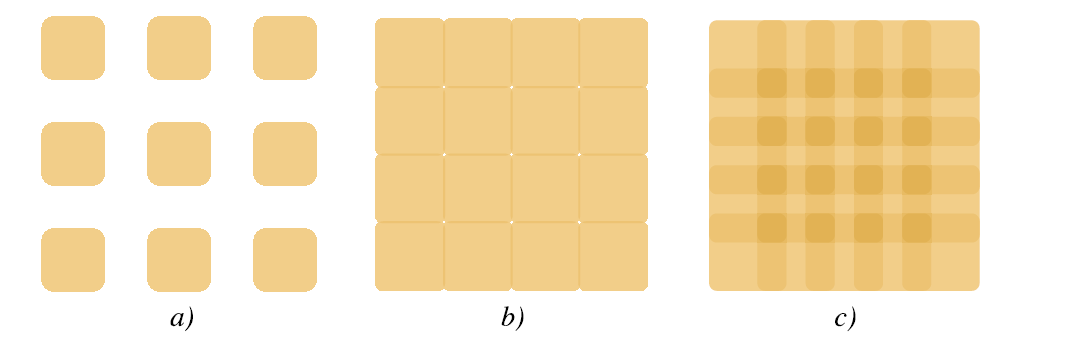
\includegraphics{images/img_17_1.PNG}
		}
		\caption{
		\label{i17.1} Спектр допустимых значений координат квантовой строки $X^\mu$. \textbf{a} $a_{\text{spacetime}}>2\pi\sqrt{\alpha\prime}$. \textbf{b} $a_{\text{spacetime}}=2\pi\sqrt{\alpha\prime}$. \textbf{c} $a_{\text{spacetime}}<2\pi\sqrt{\alpha\prime}$. Квадраты, представляющие диапазоны параметров $\eta$, были немного округлены таким образом, чтобы показать расположение возможных краевых состояний}
	\end {center}
\end {figure}

На рис.\ref{i17.1} В квантовой теории зарисовывается спектр допустимых координат пространства задания строки в квантовой теории. Только если Ик. (\ref{17.119}) точно подчиняется, классическая система точно соответствует квантовой теории, в противном случае появляются ложные пустоты или перекрытия.\footnote{Если бы размер ячейки был выбран ровно в половину от размера Eq. (\ref{17.119}), возникнет универсальный коэффициент перекрытия $2^{d-1}$, что, возможно, может быть учтено в теории суперструн.} Мы обнаружили, что наша классическая строка живет на квадратной решетке с размером ячейки $a_{\text {spacetime}}$. Согласно теории, объясненной в последних нескольких разделах этой главы, полностью квантованная бозоническая строка полностью эквивалентна этой классической строке; между ними есть двойное отображение. Условие (\ref{17.119}) на значение параметра решетки $a_{\text {spacetime}}$ является существенным для данного отображения. Если убедить теоретиков струн ограничиться координатами струн, которые живут на этой решётке, то они увидят, что полный набор квантовых состояний бозонной струны по-прежнему охватывает всё пространство Гильберта, к которому они привыкли, в то время как сейчас все базисные элементы этого пространства Гильберта распространяются классически, по дискретным аналогам классических струнных уравнений.

Интуитивно, в вышеизложенном мы приняли теорию решетки как естественную онтологическую систему, соответствующую теории невзаимодействующих струн в пространстве Минковского. Однако, в принципе, мы могли бы с тем же успехом выбрать компактифицированную теорию. Эта теория утверждала бы, что поперечные степени свободы строки живут не на $\mathbb R^{d-1}$, а на $\mathbb R^{d-1}$, a (непрерывный) тор в измерениях $d - 1$, опять же с условиями периодичности по длинам $2\pi\sqrt{\alpha\prime}$, и эти степени свободы перемещались бы
о классическом.

В секте. \ref{ch17.3.5} подробнее остановимся на природе детерминистических версий строк.


\subsubsection{The Lowest String Excitations}\label{ch17.3.3}

Теория струн - это квантовая теория поля на 1 + 1 мерном мировом листе струны. Если эта квантовая теория поля находится в своем основном состоянии, соответствующая мода струны описывает самую легкую возможную частицу в этой теории. Как только мы помещаем возбужденные состояния в теорию мирового листа, струна переходит в возбужденные состояния, что означает, что мы описываем более тяжелые частицы. Таким образом, описывается масса или энергетический спектр струны.

В первоначальных версиях теории оказалось, что самая легкая частица имеет квадрат отрицательной массы; он будет вести себя как тахион, что будет нежелательной чертой теории.
Более сложные, современные версии теории перестроены таким образом, что тахионная мода может быть объявлена нефизической, но она все еще действует как описание формального вакуума струн. Чтобы получить спектр струн, нужно начинать с этого нефизического тахионного состояния, а затем создавать описания других состояний с учетом действия операторов создания.

Чтобы связать эти струнные моды с онтологическими состояниями на детерминированных, классических сторонах нашего уравнения отображения, мы снова рассмотрим основное состояние, как это было описано в разд. \ref{ch17.1.5}, для описания тахионного решения. Таким образом, должна применяться та же процедура, что и в этом подразделе. Точно так же можно получить физические частицы, если различные операторы творения воздействуют на тахионное (основное) состояние.

Таким образом, мы получаем наше описание фотона (первое спин-одно состояние открытой струны) и гравитона (спин-2 возбужденное состояние закрытой струны).



\subsubsection{The Superstring}\label{ch17.3.4}

Для построения теорий, содержащих фермионы, было предложено установить фермионные степени свободы на мировом листе струн. Опять же, были обнаружены аномалии, если только бозонные и фермионные степени свободы не могут быть объединены в супер-мультиплеты. Каждая бозонная координата степени свободы $X ^\mu (\sigma, \tau)$ должна быть связана с фермионной степенью свободы $\psi^\mu (\sigma, \tau)$. Это должно быть сделано для левых движений независимо от правых. Дальнейший поворот в теории можно придать, только добавляя фермионные моды к левым движителям, а не к правым движителям (или наоборот); таким образом, киральность может быть введена в теорию струн, мало чем отличаясь от киральности, которая явно присутствует в Стандартной модели. Такая теория называется теорией гетеротических струн.
Поскольку мировой лист строго двумерен, у нас нет проблем со спином и спиральностью в мировом листе, поэтому здесь квантование фермионных полей - по крайней мере на уровне мирового листа - проще, чем в случае нейтрино обсуждается в разд. \ref{ch15.2.3}.

Ранее мы использовали координаты $\sigma$ и $\tau$ в качестве координат светового конуса на листе мира; теперь, временно, мы хотим использовать там пространственную и временную координаты, которые будем называть $x^{1}=x$ и $x^{0}=t$.

На листе мира спиноры являются 2-мерными, а не 4-мерными, и мы воспринимаем их как гермитианские операторы, называемые полями Майорана, которые мы пишем как

\begin{equation}\label{17.120}
\psi^{\mu *}(x, t)=\psi^{\mu}(x, t), \quad \text { and } \quad \psi^{\mu \dagger}(x, t)=\psi^{\mu * T}(x, t)
\end{equation}

(предполагая настоящее минковское целевое пространство; надписи $* T$ означают, что если $\psi=$ $\left.\left(\begin{array}{c}{\psi_{1}} \\ {\psi_{2}}\end{array}\right) \text { then } \psi^{* T}=\left(\psi_{1}^{*}, \psi_{2}^{*}\right)\right)$

Есть только две матрицы Дирака, называемые $\varrho^{0}$ и $\varrho^{1},$ или, после вращения Вика, $\varrho^{1}$ и $\varrho^{2},$ Они подчиняются...

\begin{equation}\label{17.121}
\varrho^{0}=i \varrho^{2}, \quad\left\{\varrho^{\alpha}, \varrho^{\beta}\right\}=\varrho^{\alpha} \varrho^{\beta}+\varrho^{\beta} \varrho^{\alpha}=2 \eta^{\alpha \beta}, \quad(\alpha, \beta=1,2)
\end{equation}

Полезным представлением является

\begin{equation}\label{17.121}
\varrho^{1}=\sigma_{x}=\left(\begin{array}{cc}{0} & {1} \\ {1} & {0}\end{array}\right), \quad \varrho^{2}=\sigma_{y}=\left(\begin{array}{cc}{0} & {-i} \\ {i} & {0}\end{array}\right) ; \quad e^{0}=\left(\begin{array}{cc}{0} & {1} \\ {-1} & {0}\end{array}\right)
\end{equation}

Поля-спиноры, сопряженные с полями $\psi^{\mu}(x, t)$ - это $\bar{\psi}^{\mu}(x, t),$, здесь определяемые

\begin{equation}\label{17.123}
\bar{\psi}^{\mu}=\psi^{\mu T} e^{2}
\end{equation}

Пропустив несколько незначительных шагов, касающихся фиксации колеи, которые можно найти в текстовых книгах о суперструнках, мы находим фермионную часть Лагранжа:

\begin{equation}\label{17.124}
\mathcal{L}(x, t)=-\sum_{\mu=0}^{d} \bar{\psi}^{\mu}(x, t) \varrho^{\alpha} \partial_{\alpha} \psi^{\mu}(x, t)
\end{equation}

так как $\varrho^{2}$ антисимметричные и фермионные поля антикоммутационные, два разных спинера $\psi$ и $\chi$ подчиняются.

\begin{equation}\label{17.125}
\bar{\chi} \psi=\chi^{T} \varrho^{2} \psi=i\left(-\chi_{1} \psi_{2}+\chi_{2} \psi_{1}\right)=i\left(\psi_{2} \chi_{1}-\psi_{1} \chi_{2}\right)=\psi^{T} \varrho^{2} \chi=\bar{\psi} \chi
\end{equation}

Также у нас есть

\begin{equation}\label{17.126}
\bar{\chi} \varrho^{\mu} \psi=-\bar{\psi} \varrho^{\mu} \chi
\end{equation}

антисимметрия, объясняющая, почему Лагранж (\ref{17.124}) не является чистой производной. Уравнение Дирака на листе мира строк найдено следующим образом

\begin{equation}\label{17.127}
\sum_{\alpha=1}^{2} \varrho^{\alpha} \partial_{\alpha} \psi^{\mu}=0
\end{equation}

В мире в рамке светового конуса листа пишут.

\begin{equation}\label{17.128}
\left(\varrho_{+} \partial_{-}+\varrho_{-} \partial_{+}\right) \psi=0
\end{equation}

where, in the representation (\ref{17.122})

\begin{equation}\label{17.130}
\begin{array}{l}
{\varrho^{\pm}=\frac{1}{\sqrt{2}}\left(\varrho^{0} \pm \varrho^{1}\right), \quad \text { and }} \\
{\varrho_{+}=-\varrho^{-}=\sqrt{2}\left(\begin{array}{cc}
{0} & {0} \\
{1} & {0}
\end{array}\right), \quad Q-=-\varrho^{+}=\sqrt{2}\left(\begin{array}{cc}
{0} & {-1} \\
{0} & {0}
\end{array}\right)}
\end{array}
\end{equation}

Решение уравнения (\ref{17.127}) просто

\begin{equation}\label{17.131}
\psi^{\mu}(\sigma, \tau)=\left(\begin{array}{c}
{\psi_{L}^{\mu}(\sigma)} \\
{\psi_{R}^{\mu}(\tau)}
\end{array}\right)
\end{equation}

Таким образом, обнаруживается, что фермионные левые и правые не имеют дополнительных спинорных индексов.

Как и для бозонных полей координат $X_{L, R}^{\mu}(x),$ также компоненты фермионного поля $\psi_{L, R}^{\mu}$ имеют два продольных режима, $\mu=\pm,$, которые определяются уравнениями ограничений. Эти уравнения продиктованы суперсимметрией. Так что и для фермионов мы сохраняем только поперечные компоненты $d-1$ в виде независимых динамических полей $(d$ - число пространственно-подобных размеров в целевом пространстве).

Вторая количественная теория для таких фермионных полей уже кратко обсуждалась в нашей трактовке второй количественной системы "нейтрино", в секции. \ref{ch15.2.3}. Повторим здесь, как идут дела у этих струнных фермионов из мирового листа. Опять же, мы предполагаем решетку на листе мира, в то время как уравнение Дирака на решетке теперь сводится к уравнению конечного шага, выбранному таким образом, чтобы получить точно такие же решения ( \ref{17.131}):

\begin{equation}\label{17.132}
\begin{aligned}
\psi^{i}(x, t) &=-\frac{1}{\sqrt{2}} \varrho^{0}\left(\varrho^{+} \psi^{i}(x-1, t-1)+\varrho^{-} \psi^{i}(x+1, t-1)\right) \\
i &=1, \ldots, d-1
\end{aligned}
\end{equation}


Детерминистическим аналогом является булевское множество переменных $s^{i}(x, t),$, которое, как мы предполагаем, принимает значения $\pm 1$. Можно написать их уравнение эволюции как

\begin{equation}\label{17.133}
s^{i}(x, t)=s^{i}(x-1, t-1) s^{i}(x+1, t-1) s^{i}(x, t-2)
\end{equation}

из которых решение может быть написано как

\begin{equation}\label{17.134}
s^{i}(x, t)=s_{L}^{i}(x, t) s_{R}^{i}(r, t)
\end{equation}

где $s_{L}^{i}$ и $s_{R}^{i}$ подчиняются

\begin{equation}\label{17.135}
s_{L}^{i}(x, t)=s_{L}^{i}(x+1, t-1) ; \quad s_{R}^{i}(x, t)=s_{R}^{i}(x-1, t-1)
\end{equation}

который является булевым аналогом уравнения Дирака (\ref{17.132}). Сразу видно, что все базисные элементы пространства Гильберта для уравнения Дирака могут быть отображены один к одному на состояния наших булевых переменных. Если начать с этих состояний, то существует простой способ построения операторов антикоммутирующих полей $\psi_{L, R}^{i}(x, t)$ нашей фермионики, преобразование Джордан-Вигнер $[54],$ также упоминается в Sect. \ref{ch15.2.3}. На каждое допустимое значение набора параметров $(x, i, \alpha),$, где $\alpha$ означает $L$ или $R,$ имеется оператор $a_{\alpha}^{i}(x)$, действующий на булевую переменную $s_{\alpha}^{i}(x)$ следующим образом:

\begin{equation}\label{17.136}
a|+\rangle=|-\rangle \\
a|-\rangle= 0
\end{equation}

Эти операторы и их гермитовые конъюгаты $a^{\dagger}$ подчиняются смешанным правилам борьбы с коммутацией.

\begin{equation}\label{17.137}
\left\{a_{\alpha}^{i}(x), a_{\alpha}^{i}(x)\right\}=0, \quad\left\{a_{\alpha}^{i}(x), a_{\alpha}^{i \dagger}(x)\right\}=\mathbb{I}
\end{equation}

\begin{equation}\label{17.138}
\left[a_{\alpha}^{i}\left(x_{1}\right), a_{\beta}^{j \dagger}\left(x_{2}\right)\right]=0 \quad if\\
\left\{\begin{array}{cc}{x_{1}} & {\neq x_{2}} \\ {\text { and/or }} & {i \neq j} \\ {\text { and/or }} & {\alpha \neq \beta}\end{array}\right.\\
\left[a_{\alpha}^{i}\left(x_{1}\right), a_{\beta}^{j}\left(x_{2}\right)\right]=0
\end{equation}


Включить коммутаторы в экв. (\ref{17.138}) в антикоммутаторы легко поместить весь список переменных $x, i$ и $\alpha$ в каком-то порядке. Назовем их $y$ и рассмотрим заказ $y_{1}<y_{2} .$ Затем можно определить операторы $\psi(y)$:

\begin{equation}\label{17.139}
\psi(y) \equiv\left(\prod_{y_{1}<y} s\left(y_{1}\right)\right) a(y)
\end{equation}

Это превращает правила (\ref{17.137}) и (\ref{17.138}) в антикоммутационные правила для фермионных полей:

\begin{equation}\label{17.140}
\left\{\psi\left(y_{1}\right), \psi\left(y_{2}\right)\right\}=0 ; \quad\left\{\psi\left(y_{1}\right), \psi^{\dagger}\left(y_{2}\right)\right\}=\delta\left(y_{1}, y_{2}\right)
\end{equation}

Что касается исходных переменных, то последнее правило записывается как

\begin{equation}\label{17.141}
\left\{\psi_{\alpha}^{i}\left(x_{1}\right), \psi_{\beta}^{j \dagger}\left(x_{2}\right)\right\}=\delta\left(x_{1}-x_{2}\right) \delta^{i j} \delta_{a \beta}
\end{equation}

Обозначим оставшиеся $L$ $\alpha=1$ или $\beta=1,$ и правые движки $R$ $\alpha=2$ или $\beta=2 .$ Затем выбираем нашу процедуру заказа для переменных $y_{1}=\left(x_{1}, i, \alpha\right)$ и $y_{2}=\left(x_{2}, j, \beta\right)$, которые будут определены

\begin{equation}\label{17.142}
\text { if } \alpha<\beta \text { then } y_{1}<y_{2}
\end{equation}

если $\alpha=\beta$ и $x_{1}<x_{2} \quad$, то $y_{1}<y_{2}$ если $\alpha=\beta$ и $x_{1}=x_{2}$ и $i<j$, то $y_{1}<y_{2}$ или $y_{1}=y_{2}$ или $y_{1}>y_{2}$...

Этот заказ не зависит от времени, так как все левые перемещения расположены перед всеми правыми. Следовательно, решение (\ref{17.131}) уравнения 'квантовой' дирака проходит без изменений в введенном здесь пространстве Гильберта.

Очень важно очень тщательно определить эти порядки фермионных полей, как в ураганах. (\ref{17.142}). Функция знака между скобками в экв. (\ref{17.139}), что зависит от заказа, является типичным для преобразования Джордан-Вигнер. Мы считаем, что здесь все безобидно, но это не всегда так. Такие знаковые функции могут препятствовать выполнению более сложных процедур, таких как взаимодействие между несколькими фермионами, между правым и левым движением, или в попытках перейти к более высоким измерениям (например, в $k$ -бранах, где $k>2$).

На этом этапе мы можем с уверенностью заключить, что наше двойное отображение между квантированными строками и классическими решетчатыми строками продолжает сохраняться и в случае суперструны.



\subsubsection{Детерминированные струны и продольные Моды}\label{ch17.3.5}

Поперечные моды (невзаимодействующих) квантовых бозонных и суперструн (в плоском пространстве-времени Минковского) могут быть сопоставлены с детерминированной теорией струн, движущихся вдоль целевой пространственной решетки. Как мы складываем продольные координаты и как мы проверяем инвариантность Лоренца? Правильный путь состоит в том, чтобы сначала взглянуть на квантовую теорию, где на вопросы обычно отвечают в терминах квантовых операторов.

Теперь нам действительно пришлось заменить континуум мирового листа решеткой, но мы утверждаем, что это не имеет никакого физического эффекта, потому что мы можем выбрать эту решетку так точно, как нам заблагорассудится, тогда как масштабирование мирового листа не имеет никакого влияния на физику, так как это просто преобразование координат на мировом листе. Нам действительно нужно взять лимит $\ell \rightarrow \infty$, но это, кажется, не так уж сложно.

Давайте сначала как можно больше исключим эффекты этой решетки. Перепишите Эквалайзеры. (\ref{17.5}) и (\ref{17.6}) как:

\begin{equation}\label{17.144}
\begin{aligned}
p(x, t) &=\partial_{x} k(x, t), \quad a^{L, R}(x, t)=\partial_{x} b^{L, R}(x, t) \\
b^{L}(x+t) &=k(x, t)+q(x, t) ; \quad b^{R}(x-t)=k(x, t)-q(x, t) ; \quad(17.144)
\end{aligned}
\end{equation}

the new fields now obey the equal time commutation rules $\left[q(x, t), k\left(x^{\prime}, t\right)\right]=\frac{1}{2} i \operatorname{sgn}\left(x-x^{\prime}\right)$

\begin{equation}\label{17.146}
\left[b^{L}(x), b^{L}(y)\right]=-\left[b^{R}(x), b^{R}(y)\right]=-i \operatorname{sgn}(x-y)
\end{equation}

где $\operatorname{sgn}(x)=1$ if $x>0, \operatorname{sgn}(x)=-1$ если $x<0$ и $\operatorname{sgn}(0)=0$

Оставаясь на данный момент с континуумом, мы не можем различить два "соседних" участка, поэтому не будет никакого улучшения, когда мы попытаемся заменить пограничное состояние, которое является сингулярным при $\eta(x)=\pm \pi$ на одно, которое является сингулярным, когда это значение достигается в двух соседних участках; в континууме мы ожидаем, что наши поля будут непрерывными. В любом случае, теперь мы отбросим попытку, которая дала нам выражения (\ref{17.56}) и (\ref{17.57}), но просто примем, что в каждой точке есть одно граничное состояние. Это означает, что теперь мы заменим эти уравнения отображения на

\begin{equation}\label{17.148}
b^{L}(x)=\sqrt{2 \pi} B_{\mathrm{op}}^{L}(x)+\frac{1}{\sqrt{2 \pi}} \zeta_{\mathrm{op}}^{L}(x)\\
b^{R}(x)=\sqrt{2 \pi} B_{\mathrm{op}}^{R}(x)+\frac{1}{\sqrt{2 \pi}} \zeta_{\mathrm{op}}^{R}(x)
\end{equation}

где функции $B^{L, R}$ фактически будут играть роль целых частей координат строки, а $\zeta_{\mathrm{op}}^{L, R} (x)$ определяются их действием на целочисленные функции $B^{L, R} (x),$ следующим образом:

$$
\begin{array}{ll}
{e^{i \zeta^{L}\left(x_{1}\right)}\left|\left\{B^{L, R}(x)\right\}\right\rangle=\left|\left\{B^{2, R}(x)\right\}\right\rangle,} & {\left\{\begin{aligned}
B^{\prime}^{\prime}(x)=B^{L}(x)+\theta\left(x-x_{1}\right) & \\
B^{\prime}^{\prime} R(x)=B^{R}(x) & &(17.149) \\
e^{i \zeta^{R}\left(x_{1}\right)}\left|\left\{B^{L, R}(x)\right\}\right\rangle &=\left|\left\{B^{\prime \prime L, R}(x)\right\}\right\rangle, &\left\{\begin{aligned}
B^{\prime \prime}(x)=B^{R}(x) &
\end{aligned}\right.\\
B^{\prime \prime}^{R}(x)=& B^{R}(x)+\theta\left(x_{1}-x\right)
\end{aligned}\right.}
\end{array}
$$
так что, не обращая внимания на состояние края,
$$
\left[B^{L}(x), \zeta^{L}(y)\right]=-i \theta(x-y), \quad\left[B^{R}(x), \zeta^{R}(y)\right]=-i \theta(y-x)
$$

Это дает правила коммутации (\ref{17.146}). Если мы снова рассмотрим решетку в пространстве $x$, где состояния заданы в базисе $\zeta$, то оператор $B_{\mathrm{op}}^{L} (x)$, подчиняющийся правилу коммутации (\ref{17.151}), может быть записан в виде

$$
B_{\mathrm{op}}^{L}\left(x_{1}\right)=\sum_{y<x_{1}}-i \frac{\partial}{\partial \zeta^{L}(y)}
$$

Теперь уравнение движения поперечных состояний струны ясно. Они просто разделить на левые-движители и правые двигатели, как для отдельных узлов решетки $X^{i}(\sigma, \tau)$ и для периодического $\eta^{i}(\sigma, \tau)$ функции, где $i=1, \ldots, d-1 .$ Кроме того, продольные моды разделиться на левый двигающихся те и правые двигающиеся них. Они, однако, являются фиксированными ограничениями калибровочных. В стандартной теории струн, мы можем использовать световой датчик конуса постулат, что координатный переменные $ X ^ {+} $ задаются произвольным образом по координатам мира листа, и один, как правило, выбирают уравнения связи (\ref{17.101})
Это означает, что

$$
a_{L}^{+}(\sigma)=1, \quad a_{R}^{+}(\tau)=1
$$

но простое преобразование координат $\sigma \rightarrow \sigma_{1}(\sigma)$ и $\tau \rightarrow \tau_{1}(\tau),$ можно выбрать любую другую положительную функцию координат $\sigma$ (Левый двигатель) или $\tau$ (Правый двигатель). Теперь уравнение (\ref{17.95}) здесь означает, что

$$
\left(a_{L}^{\mu}(\sigma)\right)^{2}=\left(a_{R}^{\mu}(\tau)\right)^{2}=0
$$

так что, как и в формулах. (\ref{17.102}) и $(\ref{17.103}),$ мы имеем ограничения

$$
a_{L}^{+}(\sigma)=\frac{1}{2} \sum_{i=1}^{d-1}\left(a_{L}^{i}(\sigma)\right)^{2}, \quad a_{R}^{+}(\tau)=\frac{1}{2} \sum_{i=1}^{d-1}\left(a_{R}^{i}(t)\right)^{2}
$$

где $a_{L, R}^{i}(x)=\partial_{x} b_{R, L}^{i}(x)$ (См определения \ref{17.143}). Ввиду Eq. (\ref{17.152}) для оператора $B_{L}^{i}(x),$ это теперь заманчиво писать для продольной координаты $X_{L}^{+}: \partial_{\sigma} B_{L}^{i}(\sigma)=-i \frac{\partial}{\partial \xi_{L}^{i}(\sigma)},$ так что

$$
\partial_{\sigma} X_{L}^{+}(\sigma) \stackrel{?}{=} \frac{1}{2} \sum_{i=1}^{d-1}\left(-\frac{2 \pi \partial^{2}}{\partial \zeta(\sigma)^{2}}+\frac{1}{2 \pi}\left(\partial_{\sigma} \zeta(\sigma)\right)^{2}-2 i\left\{\frac{\partial}{\partial \zeta(\sigma)}, \partial_{\sigma} \zeta(\sigma)\right\}\right),(17.156)
$$

но читатель может заметить, что теперь мы пренебрегли краевые состояния, которые здесь могут вызвать проблемы: они возникают всякий раз, когда функции $\eta^{i}$ пересекает значение $\pm \pi,$ где мы должны постулировать периодичность.

Мы видим, что мы делаем проблемы ENCOUNTER, если мы хотим, чтобы определить продольные координаты в компактифицированной классической теории поля. Кроме того, это также трудно в дискретной модели автомата, где мы только сохранить $B_{L, R}^{i},$ aS наши независимые онтологические переменные. Как мы берем их частные производные $\sigma$ и $\tau$?.

Здесь мы можем выдвинуть что калибровочные условия (17.153), возможно, придется заменить дельта-функции Дирака, с тем чтобы отразить наш выбор решетки мирового листа. Эти аспекты моделей струн мы рассматривали не хорошо изучены. Этот подраздел был добавлен, чтобы продемонстрировать кратко, что произойдет, если мы исследуем калибровочные ограничения теории, чтобы получить некоторое представление о продольных модах, в терминах онтологических состояний. На первый взгляд казалось, что компактифицировано детерминированным теория будет предлагать лучшие шансы, чтобы позволить нам строго вывести, что эти режимы похожи; кажется, что мы можем заменить решетку мирового листа на континуум, но трудности не полностью решены.

Если принять клеточный автомат на основе целых чисел $B_{L, R}^{i}$, использование решетки мирового листа практически неизбежно. На мировом листе, непрерывный предел должен приниматься с большой осторожностью.


\subsubsection{Несколько кратких замечаний о (супер) строковом взаимодействии}\label{ch17.3.6}

Пока наши (супер) строки не взаимодействуют, влияние ограничений будет незначительным. Они говорят нам, каковы координаты $X^-(\sigma,\tau)$, если мы знаем все другие координаты на мировом листе. В предыдущем разделе наша точка зрения заключалась в том, что эволюция этих координат на мировом листе является детерминированной. Наши отображения из состояний детерминированной строки в состояния квантовой строки одно, кроме краевых состояний, которые мы выбираем игнорировать. В учебниках по теории струн взаимодействия суперструн описываются с помощью топологически нетривиальных мировых листов. На практике это означает, что струны могут обмениваться руками, когда они встречаются в одной точке, или их конечные точки могут соединяться или разрываться. Все это затем контролируется струнным соединением
Рис. \ref{i17.2} Детерминированное взаимодействие струн. Это взаимодействие происходит всякий раз, когда две части строки встречаются в одной точке пространства-времени.
постоянная гс; расширение степеней gs дает строковые мировые диаграммы с последовательно более высокими топологиями.
Любопытно, что можно очень хорошо представить себе взаимодействие струн, которое является детерминированным, точно так же, как теория объема подчиняется детерминированным уравнениям. Поскольку в предыдущих разделах мы не ссылались на топологические граничные условия, мы рассматриваем детерминированное описание, полученное там, как свойство <<объема>> строки.
Естественно выглядящее взаимодействие строк будет получено, если мы постулируем следующее:
Всякий раз, когда две нити встречаются в одной точке на решетке пространства-времени, они обмениваются плечами, как показано на рис. \ref{i17.2}

\begin{figure}[ht]
	\begin{center}
		\scalebox{0.4}{
		   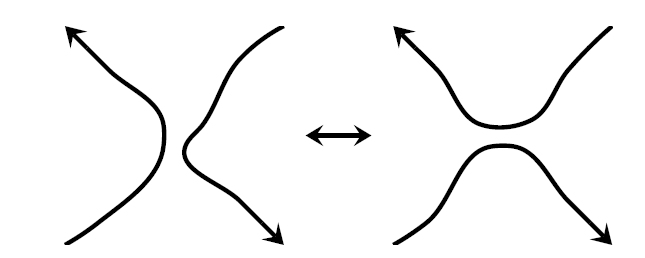
\includegraphics{images/img_17_2.png}
		}
		\caption{
		\label{i17.2} Детерминированная строка взаимодействие. Это взаимодействие происходит всякий раз, когда две части строки пересекаются в одной точке пространства-времени}
	\end {center}
\end {figure}


Этот <<закон движения>> является детерминированным и однозначным при условии, что обе строки являются ориентированными. Детерминистская версия взаимодействия не будет включать произвольно настраиваемую строковую константу $g_s$.

Если бы у нас не было проблемы, как точно определить продольные компоненты пространственно-временных координат, это завершило бы наше описание законов детерминированной струны. Теперь, однако, у нас есть проблема, что продольные координаты являются <<квантовыми>>; они получены из ограничений, которые являются нелинейными в других полях $X^\mu(\sigma,\tau)$, каждое из которых содержит целочисленные части и дробные части, которые не коммутируют. 

Эта проблема, к сожалению, значительна. Представляется, что это означает, что в терминах <<детерминированных>> переменных мы не можем точно указать, где на мировом листе происходит обмен, изображенный на рис. \ref{i17.2}. Эта трудность не была решена, поэтому пока мы не можем создать <<детерминированную>> модель взаимодействия <<квантовых>> струн.

Из нашего упражнения в теории струн мы заключаем, что струны, кажется, допускают описание в терминах онтологических объектов, но пока еще не совсем. Самые серьезные трудности лежат в продольных модах. Они нужны, чтобы понять, как теория может быть сделана лоренц-инвариантной. Так получилось, что локальная лоренцева инвариантность является проблемой для любой теории, которая пытается описать законы Природы в масштабе Планка, поэтому неудивительно, что у нас есть и эти проблемы. Мы подозреваем, что сегодняшнее неполное понимание инвариантности Лоренца в масштабе Планка необходимо исправить, но вполне может быть, что это можно сделать только в полной гармонии с интерпретацией Cellular Automaton. Этот раздел предлагает нам то, что это не может быть сделано исключительно в рамках теории струн, хотя струны могут быть полезны, чтобы привести нас к дальнейшим идеям.

Примером теории струн, которая должна быть сметена, является проблема черной дыры. Здесь также кажется, что струны захватывают физические свойства черных дыр частично, но не полностью; до тех пор, пока это так, нельзя ожидать, что мы сможем сформулировать краткую онтологическую теорию. Вот почему большинство частей этой книги концентрируются на общей философии CAI, а не на попытках построить полную модель.


\if 0


\begin{equation}\label{17.2}
	\mathcal{L}=\frac{1}{2}\left(\partial_{t} q^{2}-\partial_{x} q^{2}\right) ; \quad H_{\mathrm{op}}=\int \mathrm{d} x\left(\frac{1}{2} p^{2}+\frac{1}{2} \partial_{x} q^{2}\right)
\end{equation}

\begin{equation}\label{17.3}
	[q(x), q(y)]=[p(x), p(y)]=0 ; \quad[q(x), p(y)]=i \delta(x-y)
\end{equation}

\begin{equation}\label{17.4}
	\partial_{t}^2 q = \partial_{x}^2 q
\end{equation}

\begin{equation}\label{17.5}
	\begin{aligned} a^{L}(x, t) &=p(x, t)+\partial_{x} q(x, t)=a^{L}(x+t) \\ a^{R}(x, t) &=p(x, t)-\partial_{x} q(x, t)=a^{R}(x-t) \end{aligned}
\end{equation}

\begin{equation}\label{17.7}
	H_{\mathrm{op}}=\int \mathrm{d} x \frac{1}{4}\left(\left(a^{L}(x)\right)^{2}+\left(a^{R}(x)\right)^{2}\right)
\end{equation}

\begin{equation}\label{17.8}
	\begin{aligned}\left[a^{L}, a^{R}\right]=0, &\left[a^{L}\left(x_{1}\right), a^{L}\left(x_{2}\right)\right]=2 i \delta^{\prime}\left(x_{1}-x_{2}\right) \\ &\left[a^{R}\left(x_{1}\right), a^{R}\left(x_{2}\right)\right]=-2 i \delta^{\prime}\left(x_{1}-x_{2}\right) \end{aligned}
\end{equation}

\begin{equation}\label{17.9}
	\begin{array}{l}{a^{L, R}(k)=\frac{1}{\sqrt{2 \pi}} \int \mathrm{d} x e^{-i k x} a^{L, R}(x), \quad a^{\dagger}(k)=a(-k)} \\ {H_{\mathrm{op}}=\int_{0}^{\infty} \mathrm{d} k \frac{1}{2}\left(a^{L \dagger}(-k) a^{L}(-k)+a^{R \dagger}(k) a^{R}(k)\right)}\end{array}
\end{equation}

\begin{equation}\label{17.11}
	\begin{aligned} k, k^{\prime}>0: &\left[a^{L}\left(-k_{1}\right), a^{L}\left(-k_{2}\right)\right]=0 \\ &\left[a^{L}\left(-k_{1}\right), a^{L \dagger}\left(-k_{2}\right)\right]=2 k_{1} \delta\left(k_{1}-k_{2}\right) \\ &\left[a^{R}\left(k_{1}\right), a^{R}\left(k_{2}\right)\right]=0 \\ &\left[a^{R}\left(k_{1}\right), a^{R \dagger}\left(k_{2}\right)\right]=2 k_{1} \delta\left(k_{1}-k_{2}\right) \end{aligned}
\end{equation}

\begin{equation}\label{17.13}
	H_{\mathrm{op}}=\int_{0}^{\infty} \mathrm{d} k\left(k N^{L}(-k)+k N^{R}(k)\right)
\end{equation}

\begin{equation}\label{17.14}
	[q(x), q(y)]=\left[p^{+}(x), p^{+}(y)\right]=0 ; \quad\left[q(x), p^{+}(y)\right]=i \delta_{x, y}
\end{equation}

\begin{equation}\label{17.15}
	\begin{aligned} a^{L}(x+t) &=p^{+}(x, t)+q(x, t)-q(x-1, t) \\ a^{R}(x-t) &=p^{+}(x, t)+q(x, t)-q(x+1, t) \end{aligned}
\end{equation}

\begin{equation}\label{17.17}
	\begin{aligned}\left[a^{L}, a^{R}\right]=0 ; \quad &\left[a^{L}(x), a^{L}(y)\right]=\pm i \quad \text { if } y=x \pm 1 ; \quad \text { else } 0 ; \\ &\left[a^{R}(x), a^{R}(y)\right]=\mp i \quad \text { if } y=x \pm 1 ; \quad \text { else } 0 \end{aligned}
\end{equation}

\begin{equation}\label{17.19}
	a^{L, R}(x) \equiv \frac{1}{\sqrt{2 \pi}} \int_{-\pi}^{\pi} \mathrm{d} \kappa a^{L, R}(\kappa) e^{i \kappa x}, \quad a^{L, R \dagger}(\kappa)=a^{L, R}(-\kappa)
\end{equation}







\begin{equation}\label{17.22}
	\sqrt{2\sin k}
\end{equation}



\begin{equation}\label{17.23}
	H_{\mathrm{op}}=\int_{0}^{\pi} \mathrm{d} \kappa \frac{\kappa}{2 \sin \kappa}\left(a^{L \dagger}(-\kappa) a^{L}(-\kappa)+a^{\dagger} R(\kappa) a^{R}(\kappa)\right)
\end{equation}



\begin{equation}\label{17.24}
	a^{L}(\kappa)=p^{+}(\kappa)+\left(1-e^{-i \kappa}\right) q(\kappa), \quad a^{R}(\kappa)=p^{+}(\kappa)+\left(1-e^{i \kappa}\right) q(\kappa)
\end{equation}



\begin{equation}\label{17.25}
	H_{\mathrm{op}}=\frac{1}{2} \int_{0}^{\pi} \mathrm{d} \kappa\left(\frac{\kappa}{\tan \frac{1}{2} \kappa}\left|p^{+}(\kappa)\right|^{2}+4 k \tan \frac{1}{2} \kappa\left|q(\kappa)+\frac{1}{2} p^{+}(\kappa)\right|^{2}\right)
\end{equation}



\begin{equation}\label{17.26}
	\lim _{\kappa \rightarrow 0} \frac{\kappa}{2 \tan \left(\frac{1}{2} \kappa\right)}=1, \quad 4 \sin ^{2}\left(\frac{1}{2} \kappa\right)|q(\kappa)|^{2} \rightarrow\left|\left(\partial_{x} q\right)(\kappa)\right|^{2}
\end{equation}



\begin{equation}\label{17.27}
	\begin{aligned} \frac{\mathrm{d}}{\mathrm{d} t} a^{L}(-\kappa, t) &=-i\left[a^{L}(-\kappa, t), H_{\mathrm{op}}\right]=\frac{-i \kappa}{2 \sin \kappa} 2 \sin \kappa a^{L}(-\kappa) \\ &=-i \kappa a^{L}(-\kappa, t) \\ \frac{\mathrm{d}}{\mathrm{d} t} a^{R}(\kappa, t) &=-i \kappa a^{R}(\kappa, t) \end{aligned}
\end{equation}



\begin{equation}\label{17.28}
	\begin{aligned} a^{L}(-\kappa, t) e^{-i k x} &=a^{L}(-\kappa, 0) e^{-i \kappa x-i \kappa t} \\ a^{R}(\kappa, t) e^{i k x} &=a^{R}(\kappa, 0) e^{i \kappa x-i \kappa t} \end{aligned}
\end{equation}



\begin{equation}\label{17.29}
	a^{L}(x, 1)=a^{L}(x+1,0), \quad a^{R}(x, 1)=a^{R}(x-1,0), \quad \text { etc. }
\end{equation}



\begin{equation}\label{17.30}
	p^{+}(x, t) \equiv p\left(x, t+\frac{1}{2}\right)
\end{equation}



\begin{equation}\label{17.31}
	\begin{array}{l}{q(x, t+1)=q(x, t)+p\left(x, t+\frac{1}{2}\right)} \\ {p\left(x, t+\frac{1}{2}\right)=p\left(x, t-\frac{1}{2}\right)+q(x-1, t)-2 q(x, t)+q(x+1, t)}\end{array}
\end{equation}



\begin{equation}\label{17.33}
	H_{\mathrm{op}}=\frac{1}{2} \sum_{x, s} M_{|s|}\left(a^{L}(x) a^{L}(x+s)+a^{R}(x) a^{R}(x+s)\right)
\end{equation}



\begin{equation}\label{17.34}
	M_{s}=\frac{1}{2 \pi} \int_{-\pi+\lambda}^{\pi-\lambda} \frac{\kappa \mathrm{d} \kappa}{2 \sin \kappa} e^{-i s \kappa}=\frac{1}{2}\left\{\begin{array}{ll}{\log \frac{2}{\lambda}-\sum_{k=0}^{s / 2-1} \frac{1}{k+1 / 2}} & {\text { if } s=\mathrm{even}} \\ {\log (2 \lambda)+\sum_{k=1}^{(s-1) / 2} \frac{1}{k}} & {\text { if } s=\mathrm{odd}}\end{array}\right.
\end{equation}

\begin{equation}\label{17.35}
	\begin{array}{l}{\frac{1}{4}\left(\log \frac{1}{\lambda}\right) \sum_{x, y}(-1)^{x-y}\left(a^{L}(x) a^{L}(y)+a^{R}(x) a^{R}(y)\right)} \\ {\quad=\frac{1}{4}\left(\log \frac{1}{\lambda}\right)\left(\left(\sum_{x}(-1)^{x} a^{L}(x)\right)^{2}+\left(\sum_{x}(-1)^{x} a^{R}(x)\right)^{2}\right)}\end{array}
\end{equation}


\begin{equation}\label{17.36}
	\left(4 \kappa \tan \frac{1}{2} \kappa\right)\left(1-e^{-\Lambda^{2}(\pi-\kappa)^{2}}\right)
\end{equation}


\begin{equation}\label{17.37}
	P^{+}(x, t) \equiv P^{-}(x, t+1) \equiv P\left(x, t+\frac{1}{2}\right)
\end{equation}


\begin{equation}\label{17.38}
	\begin{array}{l}{Q(x, t+1)=Q(x, t)+P\left(x, t+\frac{1}{2}\right)} \\ {P\left(x, t+\frac{1}{2}\right)=P\left(x, t-\frac{1}{2}\right)+Q(x-1, t)-2 Q(x, t)+Q(x+1, t)}\end{array}
\end{equation}


\begin{equation}\label{17.40}
	Q(x, t+1)=Q(x-1, t)+Q(x+1, t)-Q(x, t-1)
\end{equation}


\begin{equation}\label{17.41}
	\begin{aligned} e^{-i \kappa\left(x_{1}\right)}\left|\left\{Q, P^{+}\right\}\right\rangle &=\left|\left\{Q^{\prime}(x), P^{+}(x)\right\}\right\rangle & Q^{\prime}(x) &=Q(x)+\delta_{x x_{1}} \\ e^{i \xi^{+}\left(x_{1}\right)}\left|\left\{Q, P^{+}\right\}\right\rangle &=\left|\left\{Q(x), P^{+\prime}(x)\right\}\right| ; & P^{+}(x)=P^{+\prime}(x)+\delta_{x x_{1}} \end{aligned}
\end{equation}


\begin{equation}\label{17.43}
	\begin{array}{l}{A^{L}(x, t)=P^{+}(x, t)+Q(x, t)-Q(x-1, t)} \\ {A^{R}(x, t)=P^{+}(x, t)+Q(x, t)-Q(x+1, t)}\end{array}
\end{equation}


\begin{equation}\label{17.45}
	\begin{aligned} A^{L}(x, t+1)=& P^{+}(x, t)+Q(x-1, t+1)-2 Q(x, t+1)+Q(x-1, t+1) \\ &+Q(x, t+1)-Q(x-1, t+1) \\=& P^{+}(x, t)+Q(x-1, t+1)-Q(x, t+1) \\=& P^{+}(x, t)+Q(x-1, t)+P^{+}(x-1, t)-Q(x, t)-P^{+}(x, t) \\=& P^{+}(x-1, t)+Q(x-1, t)-Q(x, t)=A^{L}(x-1, t) \end{aligned}
\end{equation}


\begin{equation}\label{17.46}
	A^{L}(x-1, t+1)=A^{L}(x, t)=A^{L}(x+t) ; \quad A^{R}(x, t)=A^{R}(x-t)
\end{equation}

\begin{equation}\label{17.47}
	\begin{aligned}\left[a^{L}, a^{R}\right]=0 ; \quad &\left[a^{L}(x), a^{L}(y)\right]=\pm i \quad \text { if } y=x \pm 1 ; \quad \text { else } 0 ; \\ &\left[a^{R}(x), a^{R}(y)\right]=\mp i \quad \text { if } y=x \pm 1 ; \quad \text { else } 0 \end{aligned}
\end{equation}



\begin{equation}\label{17.49}
	\begin{array}{ll}{e^{i \eta^{L}\left(x_{1}\right)}\left|\left\{A^{L}, A^{R}\right\}\right\rangle=\left|\left\{A^{L^{\prime}}, A^{R}\right\}\right\rangle,} & { A^{L^{\prime}}(x)=A^{L}(x)+\delta_{x, x_{1}}} \\ {e^{i \eta^{R}\left(x_{1}\right)}\left|\left\{A^{L}, A^{R}\right\}\right\rangle=\left|\left\{A^{L}, A^{R^{\prime}}\right\}\right\rangle,} & { A^{R^{\prime}}(x)=A^{R}(x)+\delta_{x, x_{1}}}\end{array}
\end{equation}



\begin{equation}\label{17.51}
	\begin{aligned} \xi(x) &=\eta^{L}(x)+\eta^{R}(x) \\-\kappa(x) &=\eta^{L}(x)+\eta^{R}(x)-\eta^{L}(x+1)-\eta^{R}(x-1) \end{aligned}
\end{equation}



\begin{equation}\label{17.52}
	\begin{array}{l}{\eta^{L}(x+1)-\eta^{L}(x-1)=\xi(x)+\kappa(x)-\xi(x-1)} \\ {\eta^{R}(x-1)-\eta^{R}(x+1)=\xi(x)+\kappa(x)-\xi(x+1)}\end{array}
\end{equation}



\begin{equation}\label{17.53}
	A e^{i \eta}=e^{i \eta}(A+1) ; \quad[\eta, A]=i
\end{equation}



\begin{equation}\label{17.54}
	\begin{array}{l}{a^{L}(x)=\sqrt{2 \pi} A^{L}(x)-\frac{1}{\sqrt{2 \pi}} \eta^{L}(x-1)} \\ {a^{R}(x)=\sqrt{2 \pi} A^{R}(x)-\frac{1}{\sqrt{2 \pi}} \eta^{R}(x+1)}\end{array}
\end{equation}



\begin{equation}\label{17.56}
	\begin{array}{l}{a^{L}(x)=-i \sqrt{2 \pi} \frac{\partial}{\partial \eta^{L}(x)}+\sqrt{2 \pi}\left(\frac{\partial}{\partial \eta^{L}(x)} \varphi\left(\left\{\eta^{L}\right\}\right)\right)-\frac{1}{\sqrt{2 \pi}} \eta^{L}(x-1)} \\ {a^{R}(x)=-i \sqrt{2 \pi} \frac{\partial}{\partial \eta^{R}(x)}+\sqrt{2 \pi}\left(\frac{\partial}{\partial \eta^{R}(x)} \varphi\left(\left\{\eta^{R}\right\}\right)\right)-\frac{1}{\sqrt{2 \pi}} \eta^{R}(x+1)}\end{array}
\end{equation}



\begin{equation}\label{17.58}
	\begin{aligned} \varphi\left(\left\{\eta^{L}(x)+2 \pi \delta_{x, x_{1}}\right\}\right.&=\varphi\left(\left\{\eta^{L}(x)\right\}\right)+\eta^{L}\left(x_{1}+1\right) \\ \varphi\left(\left\{\eta^{R}(x)+2 \pi \delta_{x, x_{1}}\right\}\right.&=\varphi\left(\left\{\eta^{R}(x)\right\}\right)+\eta^{R}\left(x_{1}-1\right) \end{aligned}
\end{equation}



\begin{equation}\label{17.60}
	\begin{array}{ll}{\phi(\kappa, \xi+2 \pi)=\phi(\kappa, \xi)+\kappa ;} & {\phi(\kappa+2 \pi, \xi)=\phi(\kappa, \xi)} \\ {\phi(\kappa, \xi)=-\phi(-\kappa, \xi)=-\phi(\kappa,-\xi) ;} & {\phi(\kappa, \xi)+\phi(\xi, \kappa)=\kappa \xi / 2 \pi}\end{array}
\end{equation}



\begin{equation}\label{17.62}
	\begin{aligned}{l}{\varphi\left(\left\{\eta^{L}\right\}\right)=\sum_{x} \phi\left(\eta^{L}(x+1), \eta^{L}(x)\right)} \\ {\varphi\left(\left\{\eta^{R}\right\}\right)=\sum_x \phi\left(\eta^{R}(x-1), \eta^{R}(x)\right)}\end{aligned}
\end{equation}


\begin{equation}\label{17.63}
	r(\kappa, \xi) e^{i \phi(\kappa, \xi)} \equiv \sum_{N=-\infty}^{\infty} e^{-\pi\left(N-\frac{\xi}{2 \pi}\right)^{2}-i N \kappa}
\end{equation}


\begin{equation}\label{17.64}
	\frac{\partial}{\partial t} \eta^{L}(x, t)=\frac{\partial}{\partial x} \eta^{L}(x, t), \quad \frac{\partial}{\partial t} \eta^{R}(x, t)=-\frac{\partial}{\partial x} \eta^{R}(x, t)
\end{equation}







\begin{equation}\label{17.69}
	\begin{aligned} \kappa^{\mathrm{op}}\left(\vec{x}, t+\frac{1}{2}\right) \text { has the same effect as } \\ & \kappa^{\mathrm{op}}\left(\vec{x}, t+\frac{3}{2}\right)-\sum_{i=1}^{2 d}\left(\xi^{\mathrm{op}}\left(\vec{x}+\hat{e}_{i}, t+1\right)-\xi^{\mathrm{op}}(\vec{x}, t+1)\right) \\ \text { and } \xi^{\mathrm{op}}(\vec{x}, t) \text { has the same effect as } \\ \quad \xi^{\mathrm{op}}(\vec{x}, t+1)-\kappa^{\mathrm{op}}\left(\vec{x}, t+\frac{1}{2}\right) \end{aligned}
\end{equation}


\begin{equation}\label{17.70}
	\xi^{\mathrm{op}}(\vec{x}, t+1)=\xi^{\mathrm{op}}(\vec{x}, t)+\kappa^{\mathrm{op}}\left(\vec{x}, t+\frac{1}{2}\right)
\end{equation}


\begin{equation}\label{17.71}
	\begin{aligned} \kappa^{\mathrm{op}}\left(\vec{x}, t+\frac{1}{2}\right)=& \kappa^{\mathrm{op}}\left(\vec{x}, t-\frac{1}{2}\right) \\ &+\sum_{i=1}^{d}\left(\xi^{\mathrm{op}}\left(\vec{x}-\hat{e}_{i}, t\right)-2 \xi^{\mathrm{op}}(\vec{x}, t)+\xi^{\mathrm{op}}\left(\vec{x}+\hat{e}_{i}, t\right)\right) \end{aligned}
\end{equation}


\begin{equation}\label{17.72}
	\begin{aligned} q^{\mathrm{op}(\vec{x}, t)} & \stackrel{?}{=} Q(\vec{x}, t)+\frac{1}{2 \pi} \xi^{\mathrm{op}}(\vec{x}, t), \quad \text { and } \\ p^{\mathrm{op}}\left(\vec{x}, t+\frac{1}{2}\right) & \stackrel{?}{=} 2 \pi P\left(\vec{x}, t+\frac{1}{2}\right)+\kappa^{\mathrm{op}}\left(\vec{x}, t+\frac{1}{2}\right) \end{aligned}
\end{equation}

\begin{equation}\label{17.73}
	\begin{array}{l}{-2 i\left(\sin \frac{1}{2} \omega\right) q(\vec{k}, \omega)=p(\vec{k}, \omega)} \\ {-2 i\left(\sin \frac{1}{2} \omega\right) p(\vec{k}, \omega)=\sum_{i=1}^{d} 2\left(\cos k_{i}-1\right) q(\vec{k}, \omega)}\end{array}
\end{equation}



\begin{equation}\label{17.74}
	4 \sin ^{2} \frac{1}{2} \omega=2(1-\cos \omega)=\sum_{i=1}^{d} 2\left(1-\cos k_{i}\right)
\end{equation}



\begin{equation}\label{17.75}
	\begin{aligned} E=& \frac{1}{2} \sum_{x} P^{+}(x, t)^{2}+\frac{1}{2} \sum_{x}\left(Q(x, t)+P^{+}(x, t)\right) \\ & \times(2 Q(x, t)-Q(x-1, t)-Q(x+1, t)) \end{aligned}
\end{equation}



\begin{equation}\label{17.76}
	E=\frac{1}{2} \int_{-\infty}^{\infty} \mathrm{d} k\left(\left(\cos \frac{1}{2} k\right)^{2}\left|P^{+}(k)\right|^{2}+4\left(\sin \frac{1}{2} k\right)^{2}\left|Q(k)+\frac{1}{2} P^{+}(k)\right|^{2}\right)
\end{equation}



\begin{equation}\label{17.77}
	
\end{equation}



\begin{equation}\label{17.}
	
\end{equation}



\begin{equation}\label{17.}
	
\end{equation}



\begin{equation}\\begin{equation}\label{17.}{17.}
	
\end{equation}

\fi













\end{document}

